\appendix

\chapter{Additional content}
\label{app:cases}

The appendix contains additional scientific case-studies as mentioned in the main thesis, along with additional arguments supporting the main content. A summary of the scientific case-studies of the appendix is shown in \cref{tab:bck-cases}. \\

\begin{table}[ht!]
\small
\centering
\begin{tabular}{p{0.15\linewidth} p{0.15\linewidth} p{0.65\linewidth}}
\hline
\textbf{Section} & \textbf{Case study} & \textbf{Narrative contribution} \\
\hline
\Cref{app:cases:monke} & monkey call detection &
We show how highly compact human-defined acoustic features can be effective for use-cases peripheral to their intended use (human speech representation), enabling small but effective models. \\
\Cref{app:cases:graph-kern} & graph kernels &
We show how feature function abstractions, specifically those implementing graph isomorphism tests, can be used to implement graph kernels. \\
\Cref{app:cases:mos}, \ref{app:cases:ppp} & speech and protein scalar property prediction &
We show how classifier confidence is a proxy for zero-shot out-of-domain detection, and that this is improved using Monte-Carlo dropout. \\
\Cref{app:cases:pb} & proximity bias &
We show how a model can drive pseudo-interpretable data analysis (to recover characteristics of and identify certain cells) in a severe data-noise regime (cell images), when model components are constrained using a scientific hypothesis. Also, as above, we show how an interpretable latent (visually striking perturbations) can be recovered from classifier confidence. \\
\Cref{app:cases:ice-cores} & ice-cores &
We show how HMMs can be significantly constrained using a priori knowledge relating to monotonicity of the latent (time), enabling interpretable recovery. \\
\Cref{app:cases:gplvm} & scRNA-seq &
We show that various data and model constraints in sparse GPLVMs, and initialisation choices drive interpretability. \\
\hline
\end{tabular}
\caption{\small Summary of scientific case studies and their contributions.}
\label{tab:bck-cases}
\end{table}

\newpage

\section{A MAP perspective on DRTree}
\label{app:cases:drtree}

In this section, we exemplify the interpretation of an objective as a log-likelihood that involves a discrete random variable, as mentioned in \cref{chp:bck-interp}.\footnote{We introduced this interpretation in \mecite{probdr}.} The DRTree \citep{drtree} algorithm finds a minimal spanning tree representation of the data, as well as projecting the data onto a low-dimensional space. The objective is written as follows,
\begin{align*}
    \mathcal{L} &= \| \Y - \X\mathbf{W} \|^2 + \dfrac{\lambda}{2} \sum_{ij} b_{ij} \| \mathbf{W}^T \X_{i:} - \mathbf{W}^T \X_{j:} \|^2 \\
    &= \text{tr}( (\Y - \X\mathbf{W})^T(\Y - \X\mathbf{W}) ) + \text{tr}(\lambda \L \X \X^T),
\end{align*}
where the second step follows as $\mathbf{W}\mathbf{W}^T$ is constrained to be $\I$. We see that the objective is approximately a negative log posterior, assuming,
\begin{align*}
    \Y | \X, \mathbf{W} &\sim \mathcal{MN}(\X\mathbf{W}, \I, \I) \\
    \X | \L &\sim \mathcal{MN}(\mathbf{0}, (\lambda \L + \beta \I)^{-1}, \I) \\
    \L &\sim \text{Uniform over tree-structured graphs}
\end{align*}
for small $\beta$ and such that $\mathbf{W} \in \text{SO}(\q)$. The optimisation occurs with respect to the joint distribution, in an alternating manner. To optimise over $\L$ given the other parameters, we maximise,
$$ \log \underbrace{p(\Y|\X, \mathbf{W})}_{c} p(\X|\L) \underbrace{p(\L)}_{\propto 1}, $$
which, ignoring the $\log\det$ term, is simply the cost of traversing all adjacencies $\sum_{ij} b_{ij} \|\mathbf{W}^T\X_i-\mathbf{W}^T\X_j\|^2$. Kruskal's algorithm finds a minimal spanning tree for the data, with known graph weights, hence we use this algorithm to find $\L$ at each step of the alternating optimisation, given the current estimates of $\X, \mathbf{W}$.

\section{The Griffin-Lim algorithm}
\label{app:cases:gla}

% fv:
% I think you should do Re for the symbol , fancy medivial looking R is a bit confusing, atm Im scrolling too much between equations and the math symbols page, you want to avoid the reader having to do this.

% fv:
% What did this probalistic interpretation bring ? I found the original GLA objective much easier to understand even though you did not explain it (please explain / give background). The probabilistic interpretation requires a lot of vectorisation , blocks / hammaering to obtain a likleihood by the time the reader has checked through the maths theyve lost the starting point so you need to remind them in very easy terms what this new interpretation adds, in the same way that papers such as pPCA do. 
% fv:
% If both your examiniers are very bayesian (i.e. do literally nothing else) then it might be fine, but if you get a more pragmatic bayesian or a non bayesian this might be a little frustrating to read. 

% 1. Give the original / initial intution / interpretaiton of the obejctive
% 2. Motivate what is lacking
% 3. State the probabilistic formulation  immediately detailing what it adds in terms of LVM interpretation

% To not tire readings and give them freedom to chose what to spend time on it might be good to also adopt a "state result first, derivation after" in a way that they can see intution / result first and then mechanistic/algebraic manipulations after

Here, we describe the GLA case-study of \cref{chp:bck-interp} in detail. In speech analysis, a common visual tool to analyse frequencies and how they change over time, is a \textbf{spectrogram}. This is typically calculated as the element-wise absolute value of a complex valued matrix known as the short-time Fourier transform (STFT) matrix. Within a STFT operation, a signal is first segmented, and a Fourier transform is computed for each segment. As an illustration,
$$ \begin{bmatrix}
    1\\ \vdots \\ 8
\end{bmatrix} \overset{\text{window}}{\longrightarrow} \begin{bmatrix} 1 & 3 & 5 \\ 2 & 4 & 6 \\ 3 & 5 & 7 \\ 4 & 6 & 8 \end{bmatrix} \underset{D\times}{\overset{\text{DFT}}{\longrightarrow}} \frac{1}{2}\begin{bmatrix} 1 & 1 & 1 & 1\\ 1 & -i & -1 & i\\ 1 & -1 & 1 & -1\\ 1 & i & -1 & -i\end{bmatrix} \begin{bmatrix} 1 & 3 & 5 \\ 2 & 4 & 6 \\ 3 & 5 & 7 \\ 4 & 6 & 8 \end{bmatrix}, $$
where $\mathbf{D}$ is the discrete Fourier transform matrix. In the example above, the number of points hopped between windows is two, and the number of points in each window is four.
% 
The inverse STFT operation obtains the real part of the inverse Fourier transform of the STFT matrix, and then performs an overlap add operation, averaging together different windows' estimates of a particular signal point. As an illustration,
$$ \text{STFT} \underset{D^{\dagger}\times}{\overset{\mathcal F^{-1}}{\longrightarrow}} \begin{bmatrix} 1 & c_2 & e_2 \\ 2 & d_2 & f_2 \\ c_1 & e_1 & 7 \\ d_1 & f_1 & 8 \end{bmatrix} \overset{\text{OLA}}{\longrightarrow} \{1, 2, \tfrac{1}{2}c_1 + \tfrac{1}{2}c_2, ...\} $$

The \textbf{Griffin-Lim algorithm (GLA)} of \cite{gla}, given the absolute value of an STFT $\S$, tries to find a complex matrix $\X = \S \odot \exp(\boldsymbol{\theta} i)$ such that the norm,
$$ \mathcal{L} = \| \mathcal{G}(\mathcal{G}^{\dagger} (\X)) - \X \|^2_F, $$
is minimised \citep{deep-gla}. Here, $\mathcal{G}$ corresponds to the short-term Fourier transform (STFT) operation, and $\mathcal{G}^{\dagger}$ corresponds to its pseudo-inverse.

For real-valued signals, the projection (taking the inverse-Fourier transform and then a Fourier transform) applied to spectrum should result in the starting spectrum, due to consistency, i.e. we expect $\mathcal{G}(\mathcal{G}^{\dagger} (\X)) = \X$. Generally, at a random initialisation of $\boldsymbol{\theta}$, the norm is non-zero due to redundant information within the STFT, as an audio sample at a specific time point contributes information to multiple windows. Therefore, not all phase matrices correspond to typical audio signals (the inverse Fourier transform must be real, the first phase is 0 for every time window, and the mirrored frequencies are the complex conjugates of the preceding frequencies, etc.). In other words, valid $\boldsymbol\theta$ occupies a small subspace of $[0, 2\pi]^{n_w\times w}$, where $n_w$ is the number of time points per window, and $w$ is the number of windows. GLA therefore, tries to minimise the disagreement between the two sides of the previous equation, by minimising the residual. The algorithm can produce perceptible speech simply from spectrogram images, and was used before the advent of large neural-vocoders. Phase reconstruction problems also appear in biological imaging.

Define $\mathbf{v} = \operatorname{vec}(\operatorname{STFT}(\mathbf{a}))$ and $\mathbf{D}_k = \I_{w}^\textsf{T} \otimes \mathbf{D}$. Further, let $\mathbf{W}$ be a repetition matrix that repeats elements of a vector such that every $n_w$ elements of the transformed vector form a window. $\mathbf{W}$ has the form,

{\tiny\begin{align*}
    \mathbf{W} =\begin{bmatrix} 1\\&1\\&&1\\&&&1\\&&1\\&&&1\\&&&&1&\cdots\end{bmatrix} \text{ and } \mathbf{W}_i = 
    \begin{bmatrix}
    1 \\
    & 1 \\
    && 0.5 && 0.5 \\
    &&& 0.5 && 0.5 \\
    &&&&&& 0.5 && 0.5 \\
    &&&&&&& 0.5 && 0.5
    \end{bmatrix}.
\end{align*}
}
Then,
\begin{align*}
\mathbf{v} = \mathcal{G}(\mathbf{a}) = \operatorname{vec}(\mathbf{D} \times \operatorname{to\_window}(\mathbf{a}) \times \I_{w}) = \mathbf{D}_k \mathbf{W} \mathbf{a}. && \text{vec-trick}
\end{align*}
Similarly, if $\mathbf{W}_i$ represents a matrix that performs the overlap-addition on a vector, one can also define the pseudo-inverse as a matrix operation,
$$ \mathbf{a} = \mathcal{G}^\dagger(\mathbf{v}) = \mathbf{W}_i \Re \left( \mathbf{D}_k^{\dagger} \mathbf{v} \right). $$
Let $\mathbf{v} = \operatorname{vec}(\S \odot \exp(\boldsymbol{\theta}i))$, $\tilde{\mathbf a} = \mathbf D_k^\dagger \mathbf{v}$ (the signal before taking the real part and overlap-adding) and $\boldsymbol{\Pi} = \mathbf{W} \mathbf{W}_i$. $\boldsymbol{\Pi}$ is symmetric and idempotent. Observe that the GLA objective can be written as,
\begin{align}
\mathcal{L} &= \| \mathbf{D}_k \mathbf{W} \mathbf{W}_i \Re \left( \mathbf{D}_k^{\dagger} \mathbf{v} \right) - \mathbf{v} \|^2_F \nonumber \\ 
&= \left\| \mathbf{D}_k\left(\mathbf{\Pi} \Re \left( \tilde{\mathbf a} \right) - \tilde{\mathbf a}  \right)\right\|^2_F \nonumber \\
&= (\mathbf{\Pi} \Re \left( \tilde{\mathbf a} \right) - \tilde{\mathbf a})^\dagger (\mathbf{\Pi} \Re \left( \tilde{\mathbf a} \right) - \tilde{\mathbf a} ) \nonumber \\
&= \Re(\tilde{\mathbf a})^T (\I - \mathbf{\Pi}) \Re(\tilde{\mathbf a}) + \Im(\tilde{\mathbf a})^T \Im(\tilde{\mathbf a}).
\label{eqn:probint:gla_qf}
\end{align}
This is the log-density\footnote{The interpretation of the loss as a complex-normal likelihood fails to provide a consistent set of parameters, as the complex normal imposes more conditions on the structure of the covariance between blocks corresponding to $\Re(\mathbf v)$ and $\Im(\mathbf v)$ than a multivariate normal would. In other words, not all PSD matrices can correspond to complex-normal precisions.} (up to constants) of the improper Gaussian with precision $\P$,
\begin{equation}
    \begin{bmatrix}
        \Re(\tilde{\mathbf a}) \\ \Im(\tilde{\mathbf a})
    \end{bmatrix} \sim
    \mathcal{N} \left(\boldsymbol{0}, \P =\begin{bmatrix}
        (\I - \mathbf{\Pi}) & \boldsymbol0 \\
        \boldsymbol0 & \I
    \end{bmatrix} \right)
\end{equation}
Consider the covariance that is implied by adding a small jitter matrix to the precision,
\begin{align*}
    \mathbf{C} &= \left( \P + \delta\I \right)^{-1} \\
    &= \begin{bmatrix}
        (1+\delta)\I - \mathbf{\Pi} & \boldsymbol0 \\
        \boldsymbol0 & (1+\delta)\I
    \end{bmatrix}^{-1}.
\end{align*}
The covariance corresponding to the imaginary part is simply $\I/(1 + \delta)$.
The covariance corresponding to the real part is,
\begin{align*}
    C_{\Re(\tilde{\mathbf{a}})\Re(\tilde{\mathbf{a}})} &= \left((1+\delta)\I - \mathbf{\Pi}\right)^{-1} \\
    &= \dfrac{1}{1+\delta} \left[ \I - \dfrac{1}{1+\delta}\mathbf{W} \left(  \dfrac{1}{1+\delta}\I -\I \right)^{-1}\mathbf{W}_i \right] && \mathbf{W}_i\mathbf{W}=\I \\
    &= \dfrac{1}{1+\delta} \left[ \I + \dfrac{1}{\delta}\mathbf{\Pi} \right].
\end{align*}
Therefore, we show that the variance for the real parts of the audio dominates the imaginary parts as $\delta \rightarrow 0$, therefore showing that the model is statistically meaningful.

\section{Effect of optimiser choice on inference}
\label{app:cases:optim}

In this section, as mentioned in \cref{subsec:gla-maintext}, we show that optimiser choice leads to difference in sparsity in recovered solutions in a logistic regression model. Concretely, in \cref{fig:optim-diffs}, we show that running gradient descent used for logistic regression, to construct a linear classifier that separates two Gaussian-distributed blobs, results in sparse solutions more often than when the Adam optimiser is used.
\begin{figure}[ht]
    \centering
    \includegraphics[width=0.5\linewidth]{figures/other_bck/adam_vs_sgd.png}
    \caption{Results of a logistic regression, i.e. the optimisation of the likelihood of a model $y_i | \mathbf{x}_i \sim \text{Bernoulli}(\sigma(\alpha x_1 + \beta x_2))$ fit to two linearly separable Gaussian blobs corresponding to two classes, in two dimensions. \textbf{Using SGD results in sparse solutions more often with respect to Adam.} Both optimisers were initialised randomly using a learning rate of 0.01 and run for 1000 epochs. The statistic visualised is the angle of the separator $\theta=\arctan(\alpha/\beta)$, and $\theta=\pi$ corresponds to a sparse solution.}
    \label{fig:optim-diffs}
\end{figure}

\section{Vocal activity detection in coppery titi monkeys}
\label{app:cases:monke}

In this section, which we briefly mention in \cref{proj:fixed}, we show a simple bioacoustics conservation case-study involving auditory representations which offer a low-dimensional frequency-domain representation of speech.\footnote{This section is based on \mecite{monke}.}

\paragraph{The problem} Actively collected acoustic data can provide valuable insights into the ecological, behavioural, and health aspects of an animal species. We focus on Coppery titi monkeys (Plecturocebus cupreus), an accessible species in local zoos. Manual processing of large volumes of acoustic data is challenging and time-consuming. The primary challenge is the development of a framework for voice activity detection using large volumes of passively collected audio containing titi monkey vocalisations, as relatively small amounts of expert-annotated data is available. Traditional methods (such as identifying segments that meet energy thresholds after passing the audio through a band-pass filter guided by the range of frequencies at which the monkeys are known to call) result in high false positives, for example, from birds that have vocal activity in the same frequency regions.

\paragraph{Available data} The dataset contains a large amount of passively collected audio data gathered in titi monkey enclosures, with a small proportion annotated by an expert. The annotations include the type of call and the start-stop times for those calls.

\paragraph{Problem representation} We treat the problem as a simple classification due to the availability of enough training data (about 3300 calls of about 0.32s duration, across 3 zoos). We assume the model,
$$y_{[t, t+\delta)}|a_{[t, t+\delta)} \sim \text{Bernoulli}(f(a_{[t, t+\delta)})),$$
where $f$ is a function acting on a segment of audio $a_{[t, t+\delta)}$, and $y_{[t, t+\delta)}$ is a label indicating whether or not the time segment contains a monkey call. We find that MFCC (Mel-frequency cepstral coefficient) representations of audio, primarily developed for human speech and introduced in \cite{mfcc}, are effective representations for our uses, despite being relatively low-dimensional and simple. MFCCs involve a lossy frequency-domain transformation of segments of audio (a discrete cosine transform of a perceptual-mapping of the segment's log-power spectrum), typically reducing a segment of a few thousand points representing the amplitudes of signals into as few as forty points representing the spectral information as it pertains to human-perceptible frequencies. Using these representations, we can then parameterise our function $f$ as a simple LSTM that acts on these base representations, and then train the model using maximum-likelihood, optimising the few parameters of the LSTM. We use a three-layer LSTM with sixteen hidden features that are linearly compressed to one scalar per window for the purposes of classification. \Cref{fig:summary:background:monke} illustrates a segment of the data, showing that expert annotations and model predictions, and that the MFCCs preserve the clusterability of distinct call types.

\paragraph{Future work} Pre-training of wav2vec2-style \citep{wav2vec2} models using the large amounts of available audio may yield better performance of our methods, as well as the use of source separation models for preprocessing the audio as part of a data-cleaning step.

\begin{figure}[ht!]
    \centering
    \includegraphics[width=0.35\linewidth]{figures/monke/monke_spec.png}
    \includegraphics[width=0.35\linewidth]{figures/monke/monke_arch.png}
    \includegraphics[width=0.7\linewidth]{figures/monke/monke_preds.png}
    \includegraphics[width=0.7\linewidth]{figures/monke/mfcc_tsne.png}
    \caption{Call detection case study. \textbf{Top left:} An illustration of a segment of audio as a spectrogram, used by domain experts to recognise and label calls. \textbf{Top right:} audio is compressed to its MFCC representation through a feature function, that is highly compressed, and can be used by a RNN that returns probability that an audio segment contains a call. \textbf{Center:} output of the RNN plotted against true labels. \textbf{Bottom:} call types visualised on a t-SNE dimensionality reduction of stretched and flattened call MFCCs, showing that MFCCs are capable of separating them.}
    \label{fig:summary:background:monke}
\end{figure}

\section{Graph embeddings}
\label{app:cases:graph-kern}

One way to featurise graph inputs, as mentioned in \cref{proj:fixed}, is to consider bit vectors consisting of substructures of the graph, visualised for a molecule in \cref{fig:chemical-secfp}. As an example, molecular fingerprints, such as the SECFP \citep{secfp}, aim to (at least in an approximate sense) solve the molecular isomorphism problem while offering low-dimensional representations of chemicals as bit vectors. Roughly, the molecular isomorphism problem, a case of the graph isomorphism problem, seeks to identify if two molecules ``are the same'' \citep{ecfp}. In graph literature, a variety of similar methods exist to tackle the graph isomorphism problem more generally, such as the Weisfeiler-Lehman approach of \cite{wl-method}, which involves the construction of a feature vector which aids the comparison of two graphs \cite{graph_kern}. Graph neural networks can be seen to generalise such featurisations \citep{wl-gnn}.

\begin{figure}
    \centering
    \includegraphics[width=0.9\linewidth]{figures/other_bck/secfp.png}
    \caption{An example of a feature function: a chemical can be represented as a bit vector, with every bit representing whether a substructure illustrated above is present.}
    \label{fig:chemical-secfp}
\end{figure}

Functions that featurise such inputs can be useful as they can be used to define kernel functions (that measure similarities between data points), used by model constructions such as Gaussian process regressors. Feature functions $\phi: \mathcal G \mapsto \mathbb R^m$ acting on graphs specifically can define kernels through the inner product, $k_{ij} = \langle \phi(\mathcal{G}_i), \phi(\mathcal{G}_j) \rangle$, leading to uncertainty measures over spaces of graphs. They can also provide a way with which to perform dimensionality reduction on graphs, using methods such as kernel PCA \citep{kpca}.

Such interpretations are helpful in software settings, as to implement graph kernels, one need only implement a feature function, and use existing abstractions (e.g. a \texttt{LinearKernel} within a \texttt{GaussianProcess} implementation). In \mecite{gauche}, we show how simple software can be written with this principle in mind within a chemical property prediction library.

\section{Mean opinion score prediction}
\label{app:cases:mos}

Many contrastive models of audio learn to classify next (latent) token from tokens randomly selected from the audio sequence. Some model frameworks follow the approach of NCE, with others following strategies similar to NCE but modifying it with information-theoretic arguments. Frameworks that describe such methods for SSL can be found in \cite{cpc, wav2vec, wav2vec2}.

We were inspired by methods in biology that use model uncertainty as a proxy scalar for property prediction, for example \cite{zero-shot-plm}, for our work in \mecite{zero-shot-mos}. We found that out-of-the-box pretrained SSL models of human audio (specifically wav2vec and wav2vec2, introduced in \cite{wav2vec, wav2vec2}) can also be used for zero-shot prediction of audio quality measured by human listeners, known as the mean-opinion score (MOS). This can be seen as an out-of-domain prediction problem, as many pretrained SSL models are trained on clean audio. The problem is tackled by measuring (a proxy of) uncertainty, such as entropy over the logits of the SSL models given a specific audio sequence as input, and using this proxy as a predictor for audio quality, with the idea that higher model uncertainty should correspond to lower quality, as lower-quality audio samples would be out-of-distribution.

Alongside the entropy, a mean of the log-probabilities is a proxy for model uncertainty as, due to the requirement that the distribution be normalised, a case of high average log-probabilities corresponds to high model uncertainty. Consider a categorical distribution with probabilities $\mathbf{p}$; as with the entropy, the quantity $\sum_i^K \log p_i$ is uniquely maximised when $\mathbf{p}$ is uniform---i.e. when the average log-probabilities are relatively high.

Graphically, the model below is hypothesised to result in a relatively good fit,
$$ y_i \longleftarrow \hat{\log p(x_i)} $$
We found that smaller models with fewer negatives (i.e. wav2vec) performed better, although the larger models could be handicapped (via feature dropout), using Monte-Carlo simulation to obtain average logits under dropout (similar to the approach of Monte-Carlo dropout, \cite{mcd}, with the caveat that our models were not trained with dropouts to begin with) to raise zero-shot performance. Performing some pre-training steps on the evaluation data, seen as domain-adaptive pre-training, also used in \cite{voice-dapt}, increased performance. 

\Cref{fig:mos-mcd} shows results of using the ideas above, obtained on the datasets provided by \cite{voicemos22, voicemos23}. The plot of SRCC (measured against the spoken English MOS ratings) of our dropout-handicapped wav2vec2 Base 960H model against dropout probability shows that performance \textbf{increases} initially as the model is handicapped.

\begin{figure}[ht]
    \centering
    \includegraphics[width=0.95\linewidth]{figures/mcd/mos_ga.png} \\
    \includegraphics[width=0.54\linewidth]{figures/mcd/mos_dp.pdf}
    \includegraphics[width=0.44\linewidth]{figures/mcd/mos_dapt.png}
    \caption{\textbf{Top:} a graphical abstract of the method, showing that an audio sample is fed to pre-trained wav2vec models, with an uncertainty measure extracted using the logits of the model. These uncertainty measures are then used as scalar proxies for property prediction at the audio level. \textbf{Bottom left:} A graph showing that injecting a dropout layer between the featuriser and the transformer layers in the wav2vec model, and calculating the logits averaged over Monte-Carlo samples under the logits increases performance initially as the dropout probability is increased. \textbf{Bottom right:} A plot showing that model performance increases when the base wav2vec model is pre-trained on (all available) evaluation data, corresponding to domain-adaptive pre-training.}
    \label{fig:mos-mcd}
\end{figure}

\section{Biochemical property prediction}
\label{app:cases:ppp}

As mentioned in \cref{proj:ssl-ood}, in \mecite{my-zeroshot-bio}, we apply the insights of dropout-averaging noted in the previous work on MOS prediction to the problem of protein fitness prediction, showing that a protein language model (ESM-2, of \cite{esm2}) zero-shot performance can be improved in a similar way for fitness prediction tasks \citep{zero-shot-plm-nature}. \cref{fig:plm-mcd} illustrates that increasing dropout and performing MCD increases zero-shot performance across all models. Future work could investigate whether the calibration of such models is indeed increased through Monte-Carlo dropout, and whether this increase in calibration driving performance boosts for scalar prediction problems.
\begin{figure}[ht]
    \centering
    \includegraphics[width=0.85\linewidth]{figures/mcd/plm_ga.png}
    \includegraphics[width=0.85\linewidth]{figures/mcd/plm_res.png}
    \caption{\textbf{Top:} Graphical abstract showing that we simply introduce a dropout between the embedding layer and transformer block of a protein language model, run many forward passes through the model and average the output log probabilities. These dropout-averaged outputs are more effective for zero-shot fitness prediction, even though the model was not trained with dropout. \textbf{Bottom:} Graphs showing the zero-shot fitness performance of ESM2 with dropout added at inference-time only.}
    \label{fig:plm-mcd}
\end{figure}

\section{Classifiers as density estimators: an LDA perspective}
\label{app:cases:lda-ood}

This section describes the idea of \cref{proj:ssl-ood} in more detail. We hypothesise that a classifier $f(\mathbf x)$ trained on data that agrees with (or is in some way robust to) the LDA assumptions follows a rule that classifier confidence decreases on average as one traverses away from the mode of the normal distribution corresponding to that class.

Explicitly, consider a two class setup, with the random variable $y$ taking values in $\{0, c\}$. Assuming LDA conditions, without loss of generality, there exists an affine transformation such that the empirical covariance of any data vector is $\I$ and such that the means of the classes sit at $\boldsymbol{0}$ and $\boldsymbol \mu_c = \{\mu_c, 0, ..., 0\}$ respectively. Focusing on the class $c$, with mean $\boldsymbol \mu_c$, we hypothesise that,
\begin{align}
    \mathbb E_{\mathbf x: \| \mathbf x - \boldsymbol \mu_c \|^2 = r^2} ( \log f(\mathbf x)) \text{ is decreasing in } r.
\end{align}
I.e. the average predicted classifier confidence drops as we move away from the cluster mode.
%
A sketch proof follows. Using the results of LDA in \cite{pml-i}, we know that,
\begin{align*}
    \hat{\mathbb P}(y=c|\mathbf{x}) &= f_c\mathbf x = \sigma(x_1 \mu_c - \mu_c^2/2) \\
    &= \sigma (z_1\mu_c + \mu_c^2/2) && \text{with } \mathbf{z} \sim \mathcal N(0, \I) \\
    \Rightarrow \mathbb E_{\mathbf x: \| \mathbf x - \boldsymbol \mu_c \|^2 = r^2} (\log f(\mathbf x)) &= \mathbb E_{\mathbf z: \| \mathbf z \|^2 = r^2} (\log \sigma (z_1\mu_c + \mu_c^2/2) ) \\
    &= \mathbb E_{\mathbf u} (\log \sigma (ru_1\mu_c + \mu_c^2/2) ) && \text{with } \mathbf u \sim \mathcal{U}: \|\mathbf u\|^2=1.
\end{align*}
We now simply show computationally in \cref{fig:lda-sim} that this function is decreasing in $r$, as the proof for this statement is tedious. The intuitive idea is that the log probability decreases towards the class boundary/linear separator faster than it increases as one moves away from the separator. Thinking of an isotropic sphere representing the data log density for a class, we can reason that on a contour of equal log-density there is a sharper fall off in the density towards the boundary than away from it.
\begin{figure}[ht]
    \centering
    \includegraphics[width=0.75\linewidth]{figures/other_bck/lda_sim.png}
    \caption{Figure showing that log confidence decreases with increasing radius in LDA.}
    \label{fig:lda-sim}
\end{figure}

We posit that these reasons provide an explanation for phenomena where classifiers can be seen to be less confident for out-of-domain examples (i.e. where the empirical data density is low), for example, as observed in \cite{class-ood}.

\section{An application of LDA in vision}
\label{app:cases:otsu}

An image segmentation algorithm, known as Otsu's method, introduced in \cite{otsu} and mentioned in \cref{proj:ssl-ood}, is an algorithm that assumes that pixel intensities in an image come from two ``classes'' causing a bi-modality in the intensity histogram. The algorithm chooses a scalar threshold along the histogram that maximises the inter-class variance of the two groups. The method is equivalent to the k-means algorithm \citep{otsu-kmeans} and therefore is related to LDA\footnote{Due to the equivalence of the k-means algorithm and EM in GMMs \citep{bishop}.}.

\begin{figure}[ht]
    \centering
    \includegraphics[width=0.9\linewidth]{figures/other_bck/nuclei_otsu.png}
    \caption{Cell nuclei segmented using Otsu thresholding, which has an LDA interpretation.}
    \label{fig:nuclei_otsu}
\end{figure}
We demonstrate the effectiveness of the method in segmentation of cellular nuclei from the JUMP cell painting dataset, specifically \href{https://cellpainting-gallery.s3.amazonaws.com/cpg0016-jump/source_13/images/20221017_Run3/images/CP-CC9-R3-15/CP-CC9-R3-15_C23_T0001F001L01A01Z01C01.tif}{an image} corresponding to the nuclear channel, of a well with cells affected by non-targeting guides used with the CRISPR-Cas9 complex. Simply applying a Gaussian filter and running the algorithm results in a clear identification of cellular nuclei, illustrated in \cref{fig:nuclei_otsu}.

\section{Misspecified data distribution in GMMs}
\label{app:cases:dcai}

\begin{figure}[ht]
    \centering
    \includegraphics[width=0.75\linewidth]{figures/other_bck/gmm_clusters.png}
    \caption{An illustration showing that the posterior probabilities over the number of clusters in a GMM is maximised with more clusters than present in the data distribution (the ground truth was two clusters), as the number of data points increases, when the generating distribution is misspecified (as Gaussian, instead of multivariate-t, which was the data generating distribution).}
    \label{fig:gmm-clusters}
\end{figure}

In this section, we illustrate the idea of \cite{dcai-gmm}, mentioned in \cref{gen:gmm}. Assume that the data generating mechanism for a real world problem is non-Gaussian and is affected by larger tails than explained by a Gaussian (which is only one of the various common misspecification types that occur in practice, along with zero inflation). Assume, for this example that a data's generating mechanism is,
\begin{align*}
k &\sim \text{Categorical}(\boldsymbol \pi), \\
\mathbf x|k &\sim \text{t}(\nu=3, \boldsymbol\mu_k, \boldsymbol\Sigma).
\end{align*}
\cite{dcai-gmm} show that, in such a scenario, if a GMM is assumed and if one uses a likelihood-based approach to determine the number of clusters present in the dataset, the true number is not recovered, and that the approach leads to an infinite number of components recovered as the number of data points increases.\footnote{Note that the Student-t is an infinite scale mixture of Gaussians.} The posterior probability of the number of classes in such an example is visualised in \cref{fig:gmm-clusters}. These probabilities are calculated using a geometric prior on the number of classes, and using the Bayesian information criterion (BIC, which is simply a linear function of the maximal log likelihood value, evaluated at the optimal mean and covariance parameters) as an approximation to the model evidence,
$$ p(k | \text{data}) \propto \exp(- \text{BIC}(k)/2)*\text{Geom}(k|r=0.01). $$
This approximation is from \cite{bic}.

\section{Proximity bias reduction}
\label{app:cases:pb}

\begin{figure}[ht]
    \centering
    \includegraphics[width=\linewidth]{figures/proxbias/pb_ga.pdf}
    \caption{Graphical abstract of the proximity bias case-study, showing (top left) a CRISPR-Cas9 complex inducing a double-strand break at a site that a guide RNA strand binds to, (top centre) the cell repairing this break, but not before some bases are lost, (top right) the cell's phenotype changing as a result as determined by images obtained using a microscope. The bottom row illustrates the computational pipeline, (bottom left) with representations first being generated, (bottom right) and a similarity matrix of gene-perturbation embeddings produced using those representations, ordered by gene position on a chromosome showing unexpected intra-chromosomal similarity.}
    \label{fig:pb-ga}
\end{figure}

In this section, we recount and expand on the results of our work in single-cell phenomics; \mecite{proxbias}. The results below follow the setup and methodology, based on \textbf{publicly available resources} (JUMP-CPG0016, \cite{cpg16}), with independently written code based on the open source release of \cite{lazar-pb}. No proprietary data, models or code were used for our presentation of ideas below.

In this section, we show how interpretable data analysis can be done, with a specific model (a Gaussian mixture model) in mind, that guides data exploration in the presence of extreme data noise. We also show how latent variables can be obtained through estimation of parameters guided through domain understanding, hence constraining the models such that useful latent variables can be recovered.

The section is organised as follows. First, we provide a biological background to explain the context of gene deletions, and the computational pipeline with which the data is analysed. We then show that this pipeline leads to an unexpected observation: correlations across representations of gene deletions within chromosome arms. We then present our work in \mecite{proxbias}, where we developed an algorithm to identify cells by minimising intra-arm correlation, and then argue that the method must be performing inference in a Gaussian mixture model. With this insight, we then discuss how such probabilistic models could be developed to recover interpretable cells in future work. Specifically, we show that a GMM with some parameters explicitly estimated using arm-averaged phenotypes and gene-averaged phenotypes reduces some amount of the unexpected correlations, and that classifier confidence can be used to measure a form of non-control-likeness that can be used for identifying visually striking perturbations.

\subsection{Biological background}

We first review the biological background of CRISPR-Cas9 induced gene deletions, and the phenomics pipelines that we are interested in.

Within the context of drug-development, understanding the behaviour of single-gene inactivations in cell lines of interest can be useful. For example, drug screens can be run to identify drugs that have a similar effect to certain known gene inactivations that have beneficial downstream effects. Additionally, single gene deletions can be helpful in discovery of biological pathways, as if two genes are on the same pathway, their single deletions can result in the same phenotype.

Experiments for such single gene deletions are done as follows. A high-throughput experimental setup is constructed, that has plates consisting of many wells in which cells of a specific kind (corresponding to certain cell-lines) are cultured. Each well holds cells which will be affected by a gene deletion, with some wells being reserved to house control cells.

Within each well, clones of a specific cell are introduced and are allowed to grow. Then, through viruses and lipofection, CRISPR-Cas9 with certain guide RNAs are introduced into cells. These complexes find a matching pattern (to the introduced guide RNA, matching portions of the gene being deleted) within DNA and induce a cut (double-strand break, DSB). The cell typically repairs such DSBs, but not before some bases at the cut-site are lost due to the activity of DNA nucleases. The loss of even a single base on the DNA can lead to the inactivation of a gene if the cut site is on an exon (a snippet used for making mRNA and subsequently protein), as a sequence of three bases corresponds to an amino acid, and a deletion of one base can lead to an entirely different amino acid being interpreted from a specific triplet of bases. Control wells typically correspond to cells infected by viruses that are non-targeting (or, in some protocols, harmlessly target introns). For each gene, and controls, multiple guides are used to ensure the deletion of a gene, and to account for variability in the effect of a gene deletion depending on where in the sequence the deletion happens (for example, it may be that deletions at the active site of some proteins would be more catastrophic to function as opposed to changes on to the surface or tail).

The typical measurement pipeline that follows for the analysis of these experiments is one where images of these cells are taken a considerable amount of time (typically days) after the infection of the viruses, to allow for time for DSBs to occur, and for their effects to take place. Some proteins have half-lives of just minutes and therefore, waiting for days allows for transcription to account for most of the protein expression in a cell. These images are fed through a pipeline that extracts representation (e.g. through human-engineered feature functions or VAEs) of gene deletions, but also accounts for variability induced by experimental artifacts (technical effects). These representations are typically centred with respect to control cells, leading to an estimate of the effect of performing an intervention corresponding to a gene deletion. Similarity matrices between gene deletion representations are constructed, which are the main objects with which gene-gene and gene-drug relationships can be studied.

These similarity matrices show something unexpected, which we present next: ``proximity-bias''.

\subsection{The proximity-bias problem}

In the previous subsection, we described how gene deletion experiments produce gene-gene similarity matrices of representations of cell images when a certain gene deletion occurs.

When the similarity matrices corresponding to representations of gene deletions are ordered by chromosome arm, we see similarities of gene embeddings within chromosome arms. This is unexpected because (due to evolutionary reasons) gene location does not generally correlate with gene function. \cite{lazar-pb} hypothesise that the reason for the unexpected correlations is due to the fact that sometimes, during cell-repair of DSBs (through the non-homologous end joining mechanism, NHEJ), megabase-scale segments of the DNA can be lost, sometimes as much as the entire chromosome arm \citep{chrom-truncs}. Such truncations are expected to occur in few cells (less than 5\%, depending on source). Such experimentally induced correlations are harmful to study true gene-gene interactions, so, in \mecite{proxbias}, we aimed to find single-cells that likely are affected by such off-target effects of using CRISPR-Cas9 for gene deletions. We term the hypothesised cells affected by these truncations ``proximity-bias (inducing) cells'' (PB cells).

In some cases, such as deletions on chromosome 17p, on which the tumour suppressor TP53 is located, deletions could induce a loss of P53 function, which is famously related to increased tumour rates, and thus, identifying PB cells is related to finding cancer-like cells in images. This pipeline is visualised in \cref{fig:pb-ga}, and a real-life similarity matrix is visualised in \cref{fig:pb-mat}.
\begin{figure}[ht]
    \centering
    \includegraphics[width=0.5\linewidth]{figures/proxbias/pb_mat.png}
    \caption{A gene-gene similarity matrix corresponding to chromosome 1, based on the CPG0016 dataset. Each element in the matrix shows the correlation of embeddings corresponding to that gene's deletion, obtained from the imaging pipeline. We see, unexpectedly, intra-arm correlation within chromosome arms, hypothesised to arise due to cells where the off-target action of CRISPR-Cas9 leads to chromosomal truncations, making some cells within chromosome arms appear similar even when they correspond to unrelated gene deletions.}
    \label{fig:pb-mat}
\end{figure}

For our work, we use the JUMP cell-painting dataset CPG0016 of \cite{cpg16}. They provide ``CellProfiler'' features \citep{cellprofiler4} available at the single-cell level, which measure statistics of cell images, for example, areas and intensities for each channel (nuclear, mitochondrial, etc.).

Assuming that, as discussed, problematic single-cells are responsible for this artefact, one can turn to unsupervised clustering methods to try to identify embeddings of a small population distinct to those of the other cells. However, in practice, cell-image embeddings carry an extreme level of variability, due to both biological and technical reasons (e.g. natural cell contortion and imaging artefacts). UMAPs performed on the single-cell embeddings show no apparent clusters. We posit that this is because such visualisations encode little information typically (encoding just a nearest-neighbour graph, in a lossy way, the information retention within which is possibly low), and a correlation matrix may encode much more information. In a sense, this provides a raison d'\^etre for methods that use the full covariance matrix instead of simply the nearest-neighbour graph.

A simple correction proposed by \cite{lazar-pb} involves subtracting an arm-specific correction such that the resulting similarities are decorrelated (with the corrections computed using gene embeddings corresponding to genes that are not expected to have a strong phenotype), but in this thesis, we detail how the underlying process can be studied.

In this subsection, we have presented the proximity bias problem as unexpected gene-gene similarities within arms, hypothetically caused due to chromosome-arm truncations that occur in some cells due to the off-target effect of CRISPR-Cas9. Next, we present a (non-probabilistic) algorithm to classify such cells.

\subsection{A cell identification algorithm}

In the previous subsection, we mention that single-cells suffering from off-target effects may cause unexpected gene-gene correlations. In this subsection, based on our work in \mecite{proxbias}, we introduce one possible method to identify the problematic PB cells. We directly try to identify single-cell representations, that when removed, reduces a loss function defined as the average intra-arm correlation. Our algorithm is shown in \cref{alg:pb-minimise}.

\begin{algorithm}
    \caption{Identifying single-cell embeddings to minimise average intra-arm correlation}
    \label{alg:pb-minimise}
    \begin{algorithmic}[1]
    \State \textbf{Input:} \\
    Raw single-cell embeddings $\mathbf{X} \in \mathbb{R}^{n \times d}$ \\
    Batch-corrected embeddings $\hat{\mathbf{X}} \in \mathbb{R}^{n \times d}$.\\
    Gene set $\mathcal{G}$ for chromosome $N$ and arm $a$.\\
    Classifier $f: \mathbb{R}^d \rightarrow \{-1, 1\}$, with params $\theta$.
    \State \textbf{Initialise:} Set initial weights $\theta_0$ and $\mathbf{w} = 1$.
    \While{not converged}
        \State Build the classification $\mathbf{w}$ by setting $q$ out of every $m$ cells with high PB score $f(\mathbf{X})$ to zero (approximately) by using softmax operations.
        \State Remove proportion of cells under percentile $p$ with lowest scores: $\mathbf{\hat{X}} = \mathbf{\hat{X}} \odot \mathbf{w}$.
        \State Group $\hat{\mathbf{X}}$ by genes in $\mathcal{G}$: $\forall g \in \mathcal{G}: \Bar{\mathbf{X}}_g = \frac{1}{|\{i: g_i = g\}|} \sum_{\{i: g_i = g\}} \hat{\mathbf{X}}_i$.
        \State Calculate correlation matrix: $\mathcal{P}(\mathbf{w}) = \text{cor}\left(\{\Bar{\mathbf{X}}_g : g \in \mathcal G\}\right)$.
        \State Set objective as mean intra-arm correlation: $\mathcal{L} = \text{mean}(\mathcal{P}(\mathbf{w}))$.
        \State Minimise; update $\theta$ by gradient descent: $\theta \leftarrow \theta - \eta \nabla \mathcal{L}(\theta)$.
    \EndWhile
    \State \textbf{Output:} Optimised classifier $f$ and binary vector $\mathbf{w}$, indicating retained cell embeddings.
    \end{algorithmic}
\end{algorithm}

We use a weakly supervised approach to filter proximity bias (``PB'') affected cells---i.e. cells corresponding to the within-arm correlations, \textit{before} aggregating single-cell embeddings. A classifier is trained to label cells as ``on-target'' or PB-affected (a latent variable) using the measurable increase in \textit{intra}-arm correlation as weak supervision. During training, the classifier minimises intra-arm similarities in aggregated gene embeddings by excluding cells.

Formally, we work with a matrix of embeddings $\hat{\mathbf{X}} \in \mathbb{R}^{n \times d}$, which contains batch-corrected $d$-dimensional embeddings of $n$ single-cells, each of which is affected by a gene perturbation $g$. The batch correction step consists of centring and scaling, meaning that the feature-wise means are exactly zero across all cells (within plates).
Our algorithm, detailed in Algorithm~\ref{alg:pb-minimise}, uses a classifier $f_\theta: \mathbb R^d \rightarrow (-1, 1)$, parameterised by $\theta$, constrained such that, in every well, a fraction of $p$ cell embeddings are chosen to be removed (i.e., set to zero). After filtering, we average embeddings by gene, and compute a gene-by-gene correlation matrix $\mathcal P$ using these embeddings, ordered by position on chromosome.

Training $f_\theta$ is difficult because we cannot backpropagate through a hypothetical discrete filtering step in order to minimise the average correlation of the gene-by-gene correlation matrix $\mathcal{P}$ with respect to $\theta$. In practice, we avoid this using a soft filtering during training. For every well we sample $m$ cells from which we aim to remove $q = \lfloor m \times p \rfloor$ cells, and average over the rest to compute our filtered embeddings. To represent the cells, we construct a set of $m$ single-cell embeddings $\mathbf{X}$, which a neural network maps to latent scores $\mathbf{Z} = f(\X) \in (-1,1)^{m\times q}$. We then calculate a soft-selection vector $\mathbf{w}$ as,
$\mathbf{w} = 1 - \min \left[ \sum_j \sigma \left(\mathcal T \mathbf{Z}_{\cdot j} \right), 1 \right],$
where $\sigma$ corresponds to the softmax function, applied column-wise (i.e. across cells) and $\mathcal T$ is an inverse-temperature hyperparameter. This construction leads to a near-discrete vector when the inverse-temperature $\mathcal{T}$ is high, and at most $q$ elements being approximately $0$, as desired.

We chose this construction over sampling using the Gumbel-softmax trick (the concrete distribution, \cite{gumbel-softmax, concrete-dist}) because we found that it led to lower variance gradients, which made the objective easier to optimise. Additionally, we found that averaging over relatively few cells (in practice we set $m$ to be 100 cells) helps us get lower variance estimates of $\mathcal{P}$ because we could load larger batches of genes into memory, leading to more stable optimisation.

\begin{figure}[ht]
    \centering
    \includegraphics[width=0.475\linewidth]{figures/proxbias/loss.png}
    \includegraphics[width=0.475\linewidth]{figures/proxbias/recall.png}
    \caption{Graphs showing that as proximity bias is reduced, recall of known biological relationships increases. These results are based on open-source resources (CPG0016, CORUM and HuMAP).}
    \label{fig:pb-res}
\end{figure}
\Cref{fig:pb-res} shows that, using a single chromosome as a proxy for the rest of the genome (as position does not generally relate to function), removing 1\% of cells within the CPG0016 embeddings leads to both a reduction in the average intra-arm correlation \textbf{and} an increase in recall of known biological relationships. To measure the latter, we used the datasets suggested by \cite{lazar-pb}, specifically the CORUM and HuMAP datasets of gene-gene relationships \citep{corum, humap}\footnote{We used the publicly available \texttt{humap2\_complexes\_20200809.txt}, where we used all complexes (with all confidence levels one through five) to form gene-gene pairs, and the publicly available \texttt{corum\_allComplexes.txt}, where we used the ``human'' complexes to form our pairs. This lead to a similar number of known relationships as \cite{lazar-pb}. We did not use the reactome dataset of \cite{reactome} as suggested by \cite{lazar-pb} as using \texttt{c2.cp.reactome.v2024.1.Hs.json} did not lead to any more unique gene-pairs.}. \mecite{proxbias} also found that the characteristics of cells removed is at least specific to chromosome arms (as a model trained on an arm cannot be used to reduce PB on another).

\textcontrib{$\star$} Unlike in the case of \mecite{proxbias}, where embeddings based on an autoencoder were used, for CPG0016 embeddings, our results are achieved only if the embeddings are first subjected to a Gaussian random projection. It may be the case that this process makes the embeddings more Gaussian-like, reducing implicit model misspecification within the algorithm. Recall of known relationships likewise is only increased when the embeddings are subjected to a Gaussian random projection.

Our objective function can be inspired by both a biological standpoint (as the inter-arm correlations are unexpected unless attributed to unintended effects of using CRISPR) but also a probabilistic perspective. In a Gaussian mixture model (where the mixtures correspond to cells affected by proximity bias and those that are not), with centred component means, the average correlation between component means naturally arises as an objective to be minimised.

To recap, we have shown an algorithm for filtering single-cells, removal of which seems to reduce proximity-bias. In the coming subsection, we argue that this inference process is approximately inference within a GMM.

\subsection{A probabilistic interpretation of correlation minimisation}

This subsection shows that assuming a Gaussian mixture model with a centred Gaussian prior over the component means, we recover an objective that penalises the average covariance between component means, which was used as a biologically-inspired heuristic in the last subsection.

\paragraph{The Model}

Consider a setting with two genes being perturbed, $a$ and $b$, located on the same chromosome arm. We assume that genetic perturbations to single-cells have a mean impact on a gene's representation with respect to control cells, measured by $\boldsymbol{\mu}^a, \boldsymbol{\mu}^b \in \mathbb R^d$. With some probability, a cell is affected by a mechanism thought to be chromosomal truncation (i.e. if a cell is ``proximally biased''), the effect of which is denoted by $\boldsymbol{\mu}^p$. We assume a multivariate Gaussian distribution on $\M$, and we assume that embeddings are centered,
$$
\M = \begin{bmatrix} {\boldsymbol{\mu}^a}^T \\ {\boldsymbol{\mu}^b}^T \\ {\boldsymbol{\mu}^p}^T \end{bmatrix}
\sim \mathcal{MN} \left( \boldsymbol{0}, (1 + \epsilon)\I - \dfrac{1}{n_g}\mathbf{O}, \I_d \right).
$$

The choice of covariance is just a centring matrix $\H$ with jitter $\epsilon$ added along the diagonal. The covariance naturally arises if we zero-centre the embeddings by construction; assume a non-zeroed normal matrix $\M'$, centring $\M'$ as $\M = \H \M'$ leads to the row-covariance $\H \I_{n_g} \H = \H$ (as $\H$ is idempotent).

If the $i$-th cell of perturbation $k$ is proximally biased, we represent it with $\mathbf{w}^k_i = 1$, and zero otherwise. The prior distribution on the vector $\mathbf{w} = [\mathbf{w}^a \quad \mathbf{w}^b]^T$ is such that, for every well (which contains $n'$ cells), exactly $\lfloor p_w n' \rfloor$ cells are sampled uniformly. This ensures that the marginal probability $\mathbb{P}(\mathbf{w}_i^k = 1)$ is $p_w$.
%
The observed control-centred representations of single-cells from the phenomics experiments are represented by $\X^a, \X^b \in \mathbb{R}^{n \times d}$. Assume that,
\begin{align*}
\X^a \mid \mathbf{w}^a, \boldsymbol{\mu}^a, \boldsymbol{\mu}^p & \sim \mathcal{MN}\left(
  (\mathbf{1} - \mathbf{w}^a) \otimes {\boldsymbol{\mu}^a}^T + \mathbf{w}^a \otimes {\boldsymbol{\mu}^p}^T,
  \sigma_m^2 \I_n, \I_d \right), \\
\X^b \mid \mathbf{w}^b, \boldsymbol{\mu}^b, \boldsymbol{\mu}^p & \sim \mathcal{MN}\left(
  (\mathbf{1} - \mathbf{w}^b) \otimes {\boldsymbol{\mu}^b}^T + \mathbf{w}^b \otimes {\boldsymbol{\mu}^p}^T,
  \sigma_m^2 \I_n, \I_d \right).
\end{align*}

\paragraph{Inference: The Objective}

The posterior is as follows,
\begin{align*}
p\bigl( \boldsymbol{\mu}^a, \boldsymbol{\mu}^b, \boldsymbol{\mu}^p, \mathbf{w} \big| \X^a, \X^b \bigr) &\propto 
p\bigl(\X \big| \M, \mathbf{w}\bigr) p\bigl(\M \bigr) p(\mathbf{w}).
\end{align*}
We use a variational approximation,
\begin{align*}
q(\mathbf{w}|\X) &= \delta(g_\theta(\X)) := \delta(\Tilde{\mathbf{w}}),
\end{align*}
where $g_\theta$ is a neural network parameterised such that its support matches that of the prior (i.e. a fixed number of cells per well are identified as proximally biased). The implied evidence lower bound (ELBO) is,
\begin{align*}
    \mathcal{L}(\theta) &= \mathbb E_{q(\mathbf{w}, \M|\X)} \left(\log p\bigl(\X \big| \M, \mathbf{w}\bigr) p(\M) \right) - \text{KL}(q(\mathbf{w}) \| p(\mathbf{w})) \\
    &= \log p(\X | \M, \Tilde{\mathbf{w}}) + \log p(\M) + c.
\end{align*}
We use block coordinate ascent for inference (i.e. CAVI/EM).
\paragraph{Inference: Step 1}
First, we maximise the objective with respect to $\M$, resulting approximately in the intuitive maximum likelihood estimator. W.l.o.g., consider the partial derivative of $\mathcal{L}(\theta)$ with respect to\ a specific component 
$\mu^a_{k}\in\mathbb{R}$, and let $\Tilde{\X^a} = \mathbf{X}^a - (\mathbf{1}-\mathbf{w}^a) \otimes {\boldsymbol{\mu}^a}^T - \mathbf{w}^a \otimes {\boldsymbol{\mu}^p}^T$. First, note that,
\begin{align*}
p\bigl(\X \big| \M, \mathbf{w} \bigr) &= p\bigl( \X^a \big| \boldsymbol{\mu}^a, \boldsymbol{\mu}^p, \mathbf{w}^a \bigr)
\cdot p\bigl( \X^b \big| \boldsymbol{\mu}^b, \boldsymbol{\mu}^p, \mathbf{w}^b \bigr),
\end{align*}
and that,
\begin{align*}
\log p(\M) &= -\dfrac{1}{2}\text{tr}\left( \M\M^T \left( (1 + \epsilon)\I - \dfrac{1}{n_g}\mathbf{O} \right)^{-1} \right) + c \\
&= -\dfrac{1}{2}\text{tr}\left( \M\M^T \left( \dfrac{1}{1 + \epsilon} \I + \dfrac{1}{\epsilon n_g(1 + \epsilon)}\mathbf{O} \right) \right) + c && \text{Sherman-Morrison} \\
&\approx -\dfrac{1}{2}\sum_{k_a} \|\boldsymbol{\mu}^{k_a}\|^2 -\dfrac{1}{2n_g\epsilon} \sum_{k_a, k_b}{\boldsymbol{\mu}^{k_a}}^T \boldsymbol{\mu}^{k_b}.
\end{align*}
%
The derivative of the ELBO with respect to a component of the mean is,
\begin{align*}
\frac{\partial}{\partial \mu^a_{k}} \mathcal{L}(\theta) &= \frac{\partial}{\partial \mu^a_{k}} \left[
\log p(\M) + \log p\bigl(\mathbf{X}^a \big|\boldsymbol{\mu}^a,\boldsymbol{\mu}^p,\mathbf{w}^a\bigr) \right] \\
&= \frac{\partial}{\partial \mu^a_{k}} \left[ \log p(\M) -\frac{1}{2\sigma_m^2} \text{tr}\Bigl[ \Tilde{\X^a} \Tilde{\X^a}^T \Bigr] - \frac{nd}{2}\log(\sigma_m^2) \right], \\
&\propto \frac{\partial}{\partial \mu^a_{k}} \left(\left[ \frac{1}{\sigma_m^2}
\sum_{i=1}^n
\Bigl\lVert \X^a_{i} - \bigl[(1 - w_i^a)\boldsymbol{\mu}^a + w_i^a\boldsymbol{\mu}^p\bigr] \Bigr\rVert^2\right] + {\mu^a_{k}}^2 + \dfrac{2 \sum_m \mu^a_k \mu^m_k}{n_g\epsilon}\right).
\end{align*}
%
Setting this derivative to $0$ for the maximum-likelihood solution leads to,
%
\begin{align*}
& 2\mu^a_{k} + \dfrac{2(2\mu^a_{k} + \mu^b_{k} + \mu^p_{k})}{n_g \epsilon} - \frac{1}{\sigma_m^2} \sum_{i=1}^n
2\bigl[X^a_{ik} - (1 - w_i^a)\mu^a_{k} - w_i^a\mu^p_{k}\bigr]
\bigl[1 - w_i^a\bigr] = 0, \\
\Rightarrow & \mu^a_{k} + \dfrac{\mu^a_{k}}{n_g \epsilon} -\frac{1}{\sigma_m^2} \sum_{i=1}^n \Bigl[X^a_{ik}(1 - w_i^a) - (1 - w_i^a)\mu^a_{k} \Bigr] = 0, \\
\Rightarrow & \mu^a_{k} + \dfrac{\mu^a_{k}}{n_g \epsilon} + \frac{n(1-p_w)\mu^a_{k}}{\sigma_m^2} - \frac{1}{\sigma_m^2} \sum_{i=1}^n \Bigl[X^a_{ik}(1 - w_i^a) \Bigr] = 0, \\
\Rightarrow & \hat{\mu}^a_{k} = \dfrac{\sum_{i=1}^n \Bigl[X^a_{ik}(1 - w_i^a) \Bigr]}{\left( \sigma_m^2 + \dfrac{\sigma_m^2}{n_g \epsilon} + n(1-p_w) \right)} \overset{n\rightarrow\infty}{\approx} \dfrac{\sum_{i=1}^n \Bigl[X^a_{ik}(1 - w_i^a) \Bigr]}{n(1-p_w)} \equiv \Bar{\X}^{a, \not p}_{:k}.
\end{align*}
We see that the solution for the mean embedding of a genetic perturbation is simply the average embedding corresponding to non-proximally biased cells known to have that perturbation induced.

\paragraph{Inference: Step 2}

In this step, we optimise the ELBO with respect to $\theta$, i.e. the parameters associated with the latent variables $\mathbf{w}$. In particular, we will argue that this step leads to minimisation of the average covariance between the average gene embeddings.

We conjecture that maximisation of $\log p(\hat{\M})$ is an important part to the optimisation of the objective $\mathcal{L}$. A sketch is as follows. The first term of the ELBO without constants (with respect to $\theta$) is,
\begin{align*}
\mathcal{T}^a_1 &\equiv -\dfrac{1}{2\sigma_m^2} \sum_{i=1}^n
\Bigl\lVert \X^a_{i} - (1 - w_i^a)\boldsymbol{\mu}^a - w_i^a\boldsymbol{\mu}^p  \Bigr\rVert^2 \\
&= -\dfrac{1}{2\sigma_m^2} \sum_{i=1}^n \sum_{k=1}^d
\left( X_{ik}^a - (1 - w^a_i)\mu^a_k - w^a_i \mu^p_k \right)^2 \\
&= -\dfrac{1}{2\sigma_m^2} \sum_{i=1}^n \sum_{k=1}^d
 (1 - w^a_i){\mu^a_k}^2 + w^a_i {\mu^p_k}^2 - 2 X_{ik}^a (1 - w^a_i)\mu^a_k - 2 X_{ik}^a w^a_i \mu^p_k + c \\
 &= \dfrac{1}{2\sigma_m^2} \sum_{k=1}^d n(1-p_w) (\Bar{\X}_{:k}^{a,\not p})^2 + np_w \Bar{\X}_{:k}^{a, p} \dfrac{\Bar{\X}_{:k}^{a, p} + \Bar{\X}_{:k}^{b, p}}{2} + c,
\end{align*}
where the last step follows from substituting the means $\mu$ with their estimates, and the fact that the mean of the perturbations will use both $\Bar{\X}_{:k}^{a, p} \text{ and } \Bar{\X}_{:k}^{b, p}$. Optimisation of this term with respect to $\theta$ (and therefore $\mathbf{w}$) should just lead to a balancing dynamic, as the relabelling of a cell would inversely affect $\Bar{\X}_{:k}^{a,\not p}$ and $\Bar{\X}_{:k}^{a,p}$.

Therefore, the optimisation of the ELBO with respect to $\theta$ should force $\log p(\hat{\M})$ upwards, which from the previous inference step is known to be inversely proportional to the average covariance between rows of $\hat{\M}$,
\begin{align*}
\log p(\hat{\M}) &= -\dfrac{1}{2n_g\epsilon} \sum_{k_a, k_b}{\boldsymbol{\mu}^{k_a}}^T \boldsymbol{\mu}^{k_b} (1 + \epsilon n_g\delta_{k_a k_b}) && \qed
\end{align*}
%
A sense-check, illustrated in figure~\ref{fig:wsl-sensecheck} verifies that average covariances are reduced by such an optimisation. We hypothesise that for our data, this proxy objective may have been a better objective than the likelihood, as our data distributions are verifiably non-normal, if there is no pathological/unanticipated behaviour being induced by the optimisation of the loss.
\begin{figure}[ht]
    \centering
    \includegraphics[width=0.5\linewidth]{figures/proxbias/wsl_sense_check.pdf}
    \caption{A sense check that confirms that the maximization of $\log \mathcal{MN}(\M' | \boldsymbol{0}, \H, \I)$ w.r.t. $\boldsymbol{\theta}$ leads to a minimization of average off-diagonal covariance between rows of $\M'$, as opposed to $\log \mathcal{MN}(\M' | \boldsymbol{0}, \I, \I)$, where the ``data'' $\M'$ is generated as $\M' = \M + p_w\tanh(\boldsymbol{\theta})$, $p_w=0.1$, and $\M$ is a Gaussian random matrix such that $\text{cor}(\M_i, \M_j) = 0.2 + 0.8\delta_{ij}$.}
    \label{fig:wsl-sensecheck}
\end{figure}

To conclude, in this subsection, we argued that a GMM underpins our objective that picks cells to minimise intra-arm correlations. In the next subsection, we show that there are features within chromosome arms that have a non-control-like distribution, and we posit that these may be the features of PB cells.

\textcontrib{\subsection{Characteristics of cells potentially causing PB}}

In the previous section, we showed that a GMM may be underpinning our method that classifies cells causing proximity-bias, by minimising intra-arm correlation. In this section, we propose a simple way to characterise them (although this has not been validated): by analysing features within arms that differ most to controls and other chromosome arms.

\begin{figure}[ht]
    \centering
    \includegraphics[width=\linewidth]{figures/proxbias/feats_by_chrom.png}
    \caption{Histograms of highly differing features by chromosome arm.}
    \label{fig:pb-feats}
\end{figure}

\Cref{fig:pb-feats} shows features that differ most by a chromosome arm with respect to the rest of the genome, standardised by the subtraction of the feature median across all genes in the genome, and scaled by the median absolute deviation (after highly zero inflated features were dropped). This method may lead to the identification of characteristics of single-cells that suffer from PB-effects as the features used here are somewhat interpretable, with the caveat that many features (co)vary together in reality, which can make joint interpretation of features difficult. Another caveat is that the features plotted are averaged across genes, and do not correspond to single-cell features. With single-cells, we therefore have a much higher noise-level.

Nevertheless, the figure highlights that arm average embeddings may identify characteristics of PB cells. One could therefore construct a GMM with arm-average embeddings to characterise PB cells, while using gene-specific embeddings to characterise non-PB cells, as we discuss in the next subsection.

\textcontrib{\subsection{Using an explicit GMM for inference}}

We find that taking one step of traditional expectation maximisation with a hard selection of the latents (respecting that only one cell out of a hundred is selected as causing PB) results in a reduction of proximity bias, when the parameters of the GMM are estimated directly using scientific heuristics. Specifically, we use a multiple (accounting for the low probability of PB-affected cells) of the average chromosome arm embedding as the expected PB embedding, and the average of embeddings corresponding to a gene perturbation as the expected non-PB embedding (as we expect few cells to be affected by PB, one would expect that this estimate would not be highly affected). This does not lead to quite as dramatic of an improvement as the algorithm derived filtering, but does lead to a meaningful difference to the amount of PB reduced, while using an interpretable method. Therefore, we propose that a refinement of the method may lead to identification of PB cells, albeit with a high false-positive rate induced by data noise.

\textcontrib{\subsection{Finding visually striking perturbations}}
\label{sec:pb-contrast}

To conclude the section, we present an observation; contrastive models can be used for finding out-of-domain examples. Using a linear classifier that has been trained to distinguish between control images and those corresponding to a single perturbation, we can define the control-likeness of a perturbation using the accuracy of the classifier as a proxy. The performance of the model is not as important here as its calibration, which is the reason behind the usage of a linear model. This leads to identification of gene deletions that are visually striking, as shown in \cref{fig:pb-ctr}. We hypothesise that many genes found in this manner are highly conserved genes, as their deletion often seems drastic to many cells in a well.
\begin{figure}[ht]
    \centering
    \includegraphics[width=\linewidth]{figures/proxbias/cell_img.png}
    \caption{Cell images, with control cells imaged on the left and perturbation on the right. This specific perturbation, clearly showing that the perturbation induces a phenotype, was found using classifier confidence, with the classifier being trained to distinguish between control cells and perturbation cells for one specific gene perturbation, using a linear model to ensure calibration.}
    \label{fig:pb-ctr}
\end{figure}

\section{Ice-cores}
\label{app:cases:ice-cores}

In this section, we detail an HMM-based model that allows for the inference of latent time as mentioned in \cref{gen:hmm}.\footnote{This section is based on \mecite{ice-cores}.} We show the versatility of such models, particularly to perform full-form inference with fine-grained assumptions such as monotonicity of the latent variable.

\begin{figure}
    \centering
    \includegraphics[width=0.66\linewidth]{figures/icecores/data.pdf}
    \includegraphics[width=\linewidth]{figures/icecores/data_recon.png}
    \includegraphics[width=0.28\linewidth]{figures/icecores/graphs.pdf}
    \includegraphics[width=0.5\linewidth]{figures/icecores/times.png}
    \caption{\textbf{Top}: The ice-cores data, chemical concentrations $s$ are a sinusoidal function of latent time, indexed by depth $\delta$. \textbf{Middle:} Predicted mean of the observation model, using the most likely sequence of latent time, using a sinusoidal generative model as part of an HMM. \textbf{Bottom left:} an illustration of the model graph used for inference, showing known concentrations $s$ being a function of latent time $t$ indexed by depth $d$. \text{Bottom right:} Latent time recovered by the HMM plotted against expert samples.}
    \label{fig:summary:background:icecores}
\end{figure}

\paragraph{Background} Ice cores preserve chemical records that reveal past climate, but extracting a reliable chronology (i.e. mapping depth to time) from these records is challenging. The traditional manual layer‐counting approach based on chemical (proxy) concentration readings is both time‐consuming and imprecise, failing to capture uncertainty in a principled manner.

\paragraph{Model} Probabilistic latent variable models, namely HMMs, lend themselves to the problem naturally \citep{mw_thesis, winstrup_hidden_2016}; the latent time process is discretised so that each depth measurement $\delta_i$ is associated with a time state $t_{\delta_i}$ taking values in $\{k/n_s: k \in \mathbb N\}$ (with $n_s$ states per annual cycle). The transition matrix is set up such that as depth increases, the time either remains in the current state or advances, and the observation model is periodic with respect to time,
\begin{align*}
\mathbb{P}(t_{\delta_i}\mid t_{\delta_{i-1}}) &= \begin{bmatrix} 
p_{1/n_s} & 1-p_{1/n_s} & 0 & \dots \\
0 & p_{2/n_s} & 1-p_{2/n_s} & \dots\\ \dots & \dots & \dots & \dots
\end{bmatrix} \\ s_{\delta_i}| t_{\delta_i} &\sim \mathcal{N}\Bigl(a\cos(2\pi t_{\delta_i})+b,\, \sigma^2\Bigr),
\end{align*}
which captures the seasonal cycle.

\paragraph{Discussion} \Cref{fig:summary:background:icecores} illustrates the data and results obtained using the model above, showing agreement between expert annotated latent time and recovered time, as well as the fit of the generative model to the chemical concentration observations. The model can be seen to perform a variant of \textbf{dynamic time warping}, but due to its probabilistic formulation, automatic inference can be performed for such use-cases using PPLs, as done in \mecite{ice-cores}. Furthermore, PPLs enable simple extensions of the model with no inference implementation overhead. For example, this allows for tie-points. These can be volcanic eruptions that deposit a layer of soot at known depths. Such events can be incorporated using a model extension that sets the expected distribution of the latent time to be uniform within the year corresponding to the eruption, at the known depth that corresponds to the eruption,
$$p(s'_{\delta_{\text{tie}}} | t_{\delta_{\text{tie}}}) = \begin{cases}
    1/n_s & \text{ if } \lfloor t_{\delta_{\text{tie}}} \rfloor = t_{\text{tie}} \\
    0 & \text{o.w.}
\end{cases}.$$ Moreover, PPLs enable inference of hierarchical variation in parameters to account for non-stationary parameters with depth (in such cases, as the MLEs lie outside the typical set, VI or MCMC is necessary as to marginalise the nuisance parameters).
% 
In the case above, as $n_s \rightarrow \infty$, the model becomes equivalent to an SDE\footnote{Specifically an SDE that can be interpreted as a monotonicity-inducing transform of a Gaussian process, as GPs have representations as stochastic differential equations, described in \cite{gp-sde}:
$$y_x \sim \mathcal{GP} \left(0, \left[1 + |x-x'|\right] \exp \left[-|x-x'| \right] \right) \Leftrightarrow \begin{bmatrix} dy_x \\ d\dot y_x \end{bmatrix} = 
    \begin{bmatrix} 0 & 1 \\ -3 & -\sqrt{12} \end{bmatrix} \begin{bmatrix} y_x \\ \dot y_x \end{bmatrix} dx + \begin{bmatrix} 0 \\ dW_x \end{bmatrix}. $$}
but inference in such a model class is difficult due to the fact that performing full-form inference for the latent path is not trivial, and parameterising the path using a function (the drift and diffusions of an SDE) leads to much worse performance.

\paragraph{Conclusion} The case study is an example of how scientifically constrained latent variable models enable the inference of interpretable latents.

\section{GPLVMs in single-cell biological data analysis}
\label{app:cases:gplvm}

\begin{figure}[ht]
    \centering
    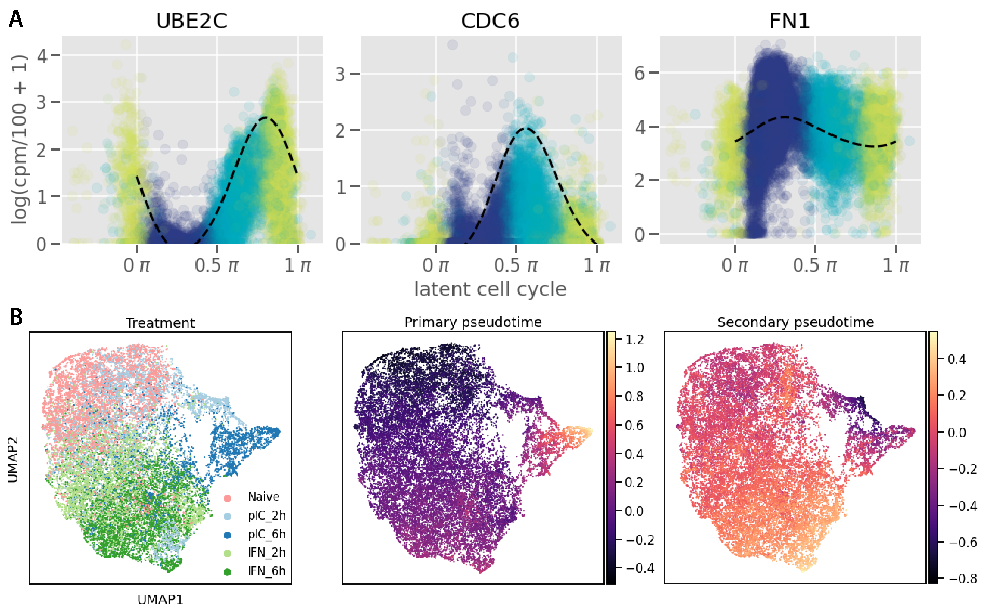
\includegraphics[width=0.7\linewidth]{figures/gplvm/nats_res.pdf}
    \caption{\textbf{Left:} Reproduction of the results of \cite{natsuhiko-paper} using our sparse extensions of GPLVMs. \textbf{Right:} 25k-dimensional gene expression projected into a 2d Poincaré disk, showing cell differentiation trajectories (coloured red to blue).}
    \label{fig:repr}
\end{figure}

\begin{figure}[ht]
    \centering
    \includegraphics[width=0.475\linewidth]{figures/gplvm/scvi.png}
    \includegraphics[width=0.475\linewidth]{figures/gplvm/gplvm.png}
    \caption{Left: a UMAP of embeddings of an scRNA-seq dataset (of \cite{covid-data}) generated using LinearSCVI of \cite{linear-scvi}. Right: a reproduction---a UMAP of the embeddings generated by interpreting LinearSCVI as a GPLVM, showing a similar disentanglement of the embeddings by cell-type and a technical variable (site).}
    \label{fig:scvi-repr}
\end{figure}

As mentioned in \cref{subsec:gplvm}, in this section, we explore how GPLVMs can be used in the context of single-cell data analysis. We briefly discuss how sparse GPLVMs are constructed, and how they are constrained in practice for the recovery of interpretable latents. We end the section by a short description of how they can be extended to non-Euclidean settings.

\paragraph{Constructing sparse GPLVMs} GPLVMs can be extended such that the GPs describing the data are made sparse \citep{gp-big-data}, which make inference on large datasets possible. \mecite{gplvm-svi} and \cite{bui-turner} show that inference in models such as,
\begin{align*}
    \Y_{ij} | \mathbf{F_{ij}} \sim \mathcal{N}(\mathbf{F}_{ij}, \sigma^2), \quad
    \mathbf{F} | \mathbf{U} &\sim \mathcal{MN}(K_{nm}K_{mm}^{-1}\mathbf{U}, K_{nn} - K_{nm}K_{mm}^{-1}K_{mn}, \I) \\
    \mathbf{U} &\sim \mathcal{MN}(\mathbf{0}, K_{mm}(\mathbf{Z}), \I),
\end{align*}
can be done variationally, with variational posteriors $q(\mathbf{U})$ and $q(\X)$ that could potentially be parameterised by neural networks.\footnote{Such variational posteriors can be specified to factorise in specific ways, for example, to respect causal ordering in temporal settings. Therefore, if one knows that a posterior decomposes in a certain way, variational posteriors can be specified to respect the factorisation, thereby narrowing the search space for the true posterior.} The ELBO \citep{blei-vi} is simply,
$$\mathcal{L} = \mathbb{E}_{q(.)}\left(\sum_{n, d} \log p(\Y_{n, d} | \mathbf{F}_{n, d})\right) - \text{KL}(q(\U) || p(\U)) - \text{KL}(q(\X) || p(\X)).$$
%
The initial motivation for our work in \mecite{gplvm-svi} was to try to fit normalising flows of \cite{flows} to the posterior to capture complex forms of uncertainty, but this is difficult due to optimisation challenges. To solve such problems on a small-data scale, we found that using a large number of Monte-Carlo samples to calculate the variational bound, \textbf{under the same random seed} (a heuristic), leads to a successful optimisation. As an example, Gaussian samples can be sampled as $\mathbf{x}=\boldsymbol{\mu} + \boldsymbol{\Sigma}^{1/2} \mathbf{z}$, where $\mathbf{z}\sim\mathcal{N}(0, \I)$ and our method samples $\mathbf{z}$ just once and keeps them fixed throughout optimisation. That being said, we noticed that such methods often resulted in a characterisation of likelihood invariance, than multi-modality due to semantically interesting uncertainty due to data-led underspecification.

\paragraph{GPLVMs in single-cell data analysis} In \mecite{tech-gplvm}, we show that frequentist GPLVMs with random effects of \cite{natsuhiko-paper} can be interpreted as \textbf{Gaussian process with linear kernels describing the random-effects}, and hence extended to their sparse counterparts (using \texttt{LinearKernel} abstractions of a sparse Gaussian process implementation) to make them scalable. The embeddings obtained are visualised in \cref{fig:repr}. The variational distributions on latents in this work are kept full-form. We found that,
\begin{enumerate}
    \item Initialisations based on PCA, covariates and marker-gene based information, with pre-identified semantic dimensions lead to identifiable latents post inference. Specifically, a latent variable corresponding to where the cell is in, within the cell-division cycle is initialised using expression of known genes that are known to be activated during certain times within the cell cycle.
    \item A periodic kernel describes the sinusoidal relationship between these latents and the expression. This imposes a strong functional constraint in the model leading to the retention of interpretable latent times, but good initialisation is crucial. Periodic covariances in such contexts have also been described, for example, by \cite{grandprix}.
    \item We also note that ``over-training'' can occur, and that continued training leads to a previously interpretable latent variable losing its interpretability.
    \item ``Pre-training'' the GPLVMs with respect to lengthscales and pseudo-inputs, with the initialisations kept frozen is needed to retain the effect of the initialisation.
    \item The pseudo-inputs can be set up in such a way that their contributions to the resulting function are independent, leading to interpretable (disentangled) inducing functions.

    As an example, consider a Gaussian process using a kernel with a linear component and an RBF-like non-linear component. Partition the inducing points $Z$ as follows,
    \begin{equation*}
        Z \equiv (Z_{\not{\text{lin}}}|Z_\text{lin}) = \begin{bmatrix}
            Z_1 & \*0 \\
            \pm \*\infty & Z_2
        \end{bmatrix}.
    \end{equation*}
    The zeros and infinities in this inducing inputs matrix are selected by considering inputs to a kernel that can set it to zero---for example, $k_{\text{rbf}}(., \pm\infty) = 0$ and $k_{\text{lin}}(., 0) = 0$. Due to this partitioning, the matrices of the sparse Gaussian process prior, $\*f | \*u \sim \mathcal N(K_{nm} K_{mm}^{-1} \*u, K_{nn} - K_{nm}K_{mm}^{-1}K_{mn}) $ simplify as follows,
\end{enumerate}
\begin{align*}
    K_{mm} &= \begin{bmatrix} k_{\not{\text{lin}}}(Z_1, Z_1) + k_\text{lin}(\*0, \*0) & k_{\not{\text{lin}}}(Z_1, \pm\*\infty) + k_\text{lin}(\*0, Z_2) \\ k_{\not{\text{lin}}}(\pm\*\infty, Z_1) + k_\text{lin}(Z_2, \*0) & k_{\not{\text{lin}}}(\pm\*\infty, \pm\*\infty) + k_\text{lin}(Z_2, Z_2) \end{bmatrix} = \begin{bmatrix} k_{\not{\text{lin}}}(Z_1, Z_1) & \*0 \\ \*0 & k_\text{lin}(Z_2, Z_2) \end{bmatrix}, \\
    K_{nm} &= \begin{bmatrix} k_{\not{\text{lin}}}(X_{\not{\text{lin}}}, Z_1) + k_\text{lin}(\Phi, \*0) & k_{\not{\text{lin}}}(X_{\not{\text{lin}}}, \pm\*\infty) + k_\text{lin}(\Phi, Z_2) \end{bmatrix} = \begin{bmatrix} k_{\not{\text{lin}}}(X_{\not{\text{lin}}}, Z_1) & k_\text{lin}(\Phi, Z_2) \end{bmatrix}.
\end{align*}
In \mecite{sarah-insights}, we found that, using the observation model, $\Y_{i:} \sim \text{Poisson}(\sigma(\mathbf{F_{i:}}) * n_l),$ (where $n_l$ denotes the library size, fixed in our experiments), preprocessing the data so that it is row normalised, and using SCVI's \citep{linear-scvi, scvi-tools} encoder (that factorises across data points, parameterising $q(\X_{i:} | \Y_{i:})$) leads to embeddings similar to that of Linear SCVI (which is equivalent to a sparse GPLVM generative model with a linear kernel). These embeddings are illustrated in \cref{fig:scvi-repr}. Moreover, we find that pretraining on cell-cycle initializations used in \cite{tech-gplvm} also recovers results of \cite{natsuhiko-paper}.

\paragraph{Non-Euclidean extensions} In \mecite{geomkerns}, we provide software for GP(LVM)s on non-Euclidean latents using kernels on manifolds and graphs \citep{matern-kern-mf, ggp}. GPLVMs specified on hyperbolic surfaces, as an example, can recover interpretable tree-structures within the data. These embeddings are illustrated in \cref{fig:hyperbolic-umap}. We hypothesise that such a choice of space also forms a strong constraint that enables recovery of interpretable latents, as in the case of hyperspheres.
\begin{figure}
    \centering
    \includegraphics[width=0.9\linewidth]{figures/gplvm/mouse_hyp.png}
    \caption{UMAPs fit on mouse epithelial data (of \cite{mouse-ti}, processed using code from \cite{ti-course}) with a hyperbolic kernel, showing how undifferentiated cells are more likely to be found near the origin of the UMAP, thereby exposing the underlying tree-structure of the data.}
    \label{fig:hyperbolic-umap}
\end{figure}

\paragraph{Conclusion} The examples of this section exemplify how \textbf{constraints} placed within GPLVMs, that otherwise have large degrees of freedom, are useful in practice.

\section{Embeddings in CNE following SGNS-style arguments}
\label{app:cases:sgns}

For this algorithm, following from our exposition in \cref{probdr:sgns}, we use a heuristically modified adjacency matrix. The modification involves raising our adjacency matrix to the power $r$ (selected so that all adjacencies are non-zero) that has a similar degree (achieved by multiplying the normalised adjacency with the desired degree $k$),
$$\Tilde{\A} = k (\mathbf{D}^{-1/2}\A\mathbf{D}^{-1/2})^{r}. $$
\Cref{fig:sgns-tsne} illustrates an embedding of the MNIST dataset obtained by the arguments above. The resulting embedding is a ``smoother'' version of Laplacian Eigenmaps, however, it fails to achieve the amount of separation of clusters achieved by CNE.\footnote{The style of our approximation is similar in form to SGNS-inspired matrix-factorisation results interpreting node2vec and similar algorithms \citep{node2vec-sgns}.}
\begin{figure}
    \centering
    \includegraphics[width=0.5\linewidth]{figures/probdr/mnist_sgns.png}
    \caption{An MNIST embedding obtained as an approximate solution to the CNE objective, using an eigendecomposition of an element-wise function applied to the adjacency matrix. This element-wise function results from a pairwise stationarity analysis of the CNE objective, and is inspired by the work of \cite{sgns-svd} in the context of word2vec/SGNS. The resulting embedding is more diffuse than Laplacian Eigenmaps, but with clusters that are not quite as well separated as in CNE, t-SNE or UMAP.}
    \label{fig:sgns-tsne}
\end{figure}

%%%%%%%%%%%%%%%%%%%%%%%%%%%%%%%%%%%%%
%
%
%
%
%
%
%
%
%%%%%%%%%%%%%%%%%%%%%%%%%%%%%%%%%%%%%%

\chapter{Additional proofs}

\section{Noise levels in dp-PCA and dp-MCA}
\label{app:proofs:noise-lvl}

\begin{proof} of \cref{thm:beta_vs_sigma_sq}.
Assume the setup of \cref{thm:mca_pca_equiv} and let $\lambda$s be major eigenvalues of the sample covariance matrix. Due to \cref{thm:pca}, \cref{thm:mca}, and the fact that the major eigenvalues of the sample covariance are minor eigenvalues of the precision,
$$ \hat{\sigma}^2 = \frac{\sum_{i=\q+1}^{n} \lambda_i}{n - \q} \text{ and } \hat{\beta} =  \frac{n - \q}{\sum_{i=\q+1}^{n} \dfrac{1}{\lambda_i}}. $$
%
Therefore,
\begin{align*}
    \dfrac{\hat{\sigma}^2}{\hat{\beta}} &= \dfrac{ \sum_{i=\q+1}^{n} 1/\lambda_i \sum_{i=\q+1}^{n} \lambda_i }{(n - \q)^2} \overset{\text{AM-GM}}{\geq} \sqrt[n-\q]{\prod_i \lambda_i/\lambda_i} = 1.
\end{align*}
\end{proof}

\section{The derivation of our CNE objective}
\label{app:proofs:cne}

This section shows how the CNE bound of \cref{subsec:cne} is derived.

Note that we've made some substitutions in the original formation that appears in \cite{nc_sne}, for example, we set their parameter $\Tilde{q}_{ij} = 1/d_{ij}^2$, which corresponds to the UMAP setting. Eqn. 8 of \cite{nc_sne} reads,
$$\mathcal{L}^{\text{NEG}}(\theta) = -\mathbb{E}_{x\sim p} \log \left( \dfrac{q_\theta(x)}{q_\theta(x) + 1} \right) - m \mathbb E_{x \sim \xi} \log \left( 1 - \dfrac{q_\theta(x)}{q_\theta(x) + 1} \right).$$
We use the notation $n_{\text{neg}} = m$, and we consider the objective (resulting in \cref{eqn:cne-bound}) in terms of the negative loss $\mathcal E = -\mathcal L$. Next, Lemma 3 of \cite{nc_sne} specifies the choice of $q_\theta$ corresponding to UMAP to be $q_\theta(x) = 1/d_{ij}^2(\X)$. The objective simplifies to,
\begin{align*}
\mathcal{E}(\X) &= \dfrac{1}{\sum_{i>j} \A_{ij}} \sum_{i>j} \A_{ij} \log \left( \dfrac{1}{1 + d_{ij}^2(\X)} \right) + \dfrac{n_{\text{neg}}}{\sum_{i>j} (1 - \A_{ij})} \sum_{i>j} (1 - \A_{ij}) \log \left( 1 - \dfrac{1}{1 + d_{ij}^2(\X)} \right) \\
&\propto \sum_{i>j} \A_{ij} \log \left( \dfrac{1}{1 + d_{ij}^2(\X)} \right) + \dfrac{n_{\text{neg}} \sum_{i>j} \A_{ij}}{\sum_{i>j} (1 - \A_{ij})} \sum_{i>j} (1 - \A_{ij}) \log \left( 1 - \dfrac{1}{1 + d_{ij}^2(\X)} \right)
\end{align*}
The multiplicative constant is approximated as,
\begin{align*}
\Tilde{\epsilon} &:= \dfrac{n_{\text{neg}}\sum_{i>j}\A_{ij}}{\sum_{i>j}1 - \A_{ij}} \approx \dfrac{n*n_{\text{neg}}* n_{\text{neigh}}/1.5}{(n^2 - n)/2} \approx \dfrac{4n_{\text{neg}} n_{\text{neigh}}}{3n}.
\end{align*}
Therefore, the objective becomes,
\begin{align*}
\mathcal{E}(\X) &\approx \sum_{i>j} \A_{ij} \log \left( \dfrac{1}{1 + d_{ij}^2(\X)} \right) + \dfrac{4n_{\text{neg}} n_{\text{neigh}}}{3n} \sum_{i>j} (1 - \A_{ij}) \log \left( 1 - \dfrac{1}{1 + d_{ij}^2(\X)} \right) \\
&\propto \sum_{ij} \A_{ij} \log \left( \dfrac{1}{1 + d_{ij}^2(\X)} \right) + \dfrac{4n_{\text{neg}} n_{\text{neigh}}}{3n} \sum_{ij} (1 - \A_{ij}) \log \left( 1 - \dfrac{1}{1 + d_{ij}^2(\X)} \right),
\end{align*}
which is \cref{eqn:cne-bound}.

\textcontrib{\section{On semantic consistency}}
\label{app:proofs:wish-consistent}

In this section, as mentioned in \cref{probdr:nonlin-wish}, we show that the assumptions that underpin our Wishart interpretation are semantically consistent, i.e. correspond to natural assumptions given the data structures being modelled. We also provide a possible reason for why interpreting a Wishart distribution from a multivariate Bernoulli is successful. We show these results to reiterate claim made in the introduction that the different model choices in ProbDR ``translate'' as expected. The first subsection explores the Wishart interpretation, while the latter considers how our Wishart model can be translated to one directly comparable to GPLVM (i.e. we consider what happens when the distribution on the data covariance is changed from inverse-Wishart to Wishart).

\textcontrib{\subsection{Consistency of the Wishart interpretation}}

Consider the non-linear ProbDR model,
\begin{align*}
    \L | \X \sim \mathcal{W} \left((0.5\Tilde{\epsilon}^{-1}\I + 0.5 \H \P^u \H + \X \X^T)^{-1}, n \right).
\end{align*}
%
Assume that the posterior variance corresponds to the marginals $\text{Var}(\X_i|\L) = \sigma_x^2 \I$. This is more or less a reasonable assumption, as ignoring the kernel term results in the Laplacian Eigenmaps solution, with the MAP embedding found at the scaled eigenvectors of $\L/n$, which are orthonormal.  Hence, the assumption made simply assumes that the top eigenvalues are of comparable scale\footnote{and are approximately the algebraic connectivity---although this can be approximated for Erd\Hungarian{o}s–R\'enyi graphs, an approximation for kNN graphs is likely difficult to find, as these graphs have substantially different properties. For example, degrees of a kNN graph are guaranteed to be between the number of nearest neighbours or twice that number, the latter simply due to the symmetrisation of the graph adjacency.}.

A way to see that the relationship between a kernel term $p$ and a term of the data denoted here as $\mathcal D$ is preserved between the Bernoulli and Wishart interpretations is that, within natural exponential families of the form (written in terms of the natural parameter),
$$ \log p(\boldsymbol{\mathcal{D}} |\mathbf{p}) = \boldsymbol\eta^T\boldsymbol{\mathcal{D}} - A(\boldsymbol\eta), $$
The properties of the log-partition function imply that \citep{expfam-wainwright},
\begin{align*}
    \mathbb E(\boldsymbol{\mathcal{D}}) = \nabla_{\boldsymbol{\eta}} A(\boldsymbol{\eta}) \text{ and } \text{Cov}(\boldsymbol{\mathcal{D}}) = \nabla_{\boldsymbol{\eta}} \nabla_{\boldsymbol{\eta}}^T A(\boldsymbol{\eta}) \succeq 0.
\end{align*}
The second condition implies directly that $\text{diag}(\nabla_{\boldsymbol{\eta}} \mathbb E(\boldsymbol{\mathcal D})) \geq \mathbf 0 $, meaning that the mean of the data $\boldsymbol{\mathcal D}$ is monotonic increasing in the natural parameter $\boldsymbol{\eta}$. With the Bernoulli and Poisson interpretations, the likelihood term has a positive sign, and the adjacency is described as having a mean that is increasing in the probability parameter. With the Wishart interpretations, the sign of the likelihood is negative, and hence the mean of the random variable describing the graph Laplacian is a decreasing function of the probabilities, which is semantically consistent, as the off-diagonal elements of the graph Laplacian describe \textbf{negative} adjacency.

This argument can be made explicitly, and for this, we will derive an approximation of the precision matrix of a kernel matrix. The Cauchy kernel can be expressed in terms of random Fourier features described in \cite{rff},
\begin{align*}
    \mathbf K \approx \mathbf{\Phi\Phi^T}, \mathbf\Phi \in \mathbb R^{n \times m} \text{ with } \mathbf{\Phi}_{ij} = \sqrt{\dfrac{2}{m}} \cos(\X_i^T \boldsymbol{\Omega}_j + \mathbf{b}_j).
\end{align*}
%
Let the covariance of our interpretation in \cref{eqn:wish-interp} be,
$$ \mathbf{\Sigma} = \X\X^T + 0.5 \mathbf{K} + \beta \I = ( \X \enspace \sqrt{0.5} \boldsymbol\Phi ) ( \X \enspace \sqrt{0.5} \boldsymbol\Phi )^T + \beta \I := \Tilde{\boldsymbol\Phi} \Tilde{\boldsymbol\Phi}^T + \beta \I, $$
where we drop the double centring of $\mathbf K$, which does not negatively impact the quality of the visualisations after optimisation, and $\beta = 1/2\Tilde{\epsilon}$. Using Woodbury, we see that,
\begin{align*}
    \mathbf{\Sigma}^{-1} &= 2\Tilde{\epsilon} \I - 4\Tilde{\epsilon}^2 \Tilde{\boldsymbol\Phi} \M \Tilde{\boldsymbol\Phi}^T \text{ where,} \\
    \M^{-1} &= \I + 2\Tilde{\epsilon}\boldsymbol{\Tilde{\Phi}}^T\boldsymbol{\Tilde{\Phi}} \\
    &= \begin{bmatrix}
        \I_q + 2\Tilde{\epsilon}\X^T\X & 2\sqrt{0.5}\Tilde{\epsilon} \X^T\boldsymbol{\Phi} \\
        2\sqrt{0.5}\Tilde{\epsilon} \boldsymbol{\Phi}^T\X & \I_m + \Tilde{\epsilon}\boldsymbol{\Phi}^T\boldsymbol{\Phi}
    \end{bmatrix}
\end{align*}
%
The role of $\M^{-1}$ coarsely is one that (a) behaves as a factor $\M^{-1} = \boldsymbol\Theta(n\Tilde{\epsilon}) = \boldsymbol\Theta(1)$ and (b) is otherwise a function of feature correlations. Using these results,
$$\mathbb E(\L_{ij}|\X) \sim \text{d.o.f.} * \boldsymbol\Sigma^{-1}_{ij} \sim -n\Tilde{\epsilon}^2 \sim -1/n, $$
as expected of the graph Laplacian.

Although we do not detail the computation here, $\M^{-1}$ can be approximated well using standard algebra, assuming that $\X|\L \sim \mathcal{MN}(0, \Sigma, \I_\q)$. This leads to an \textbf{approximation of a Gaussian process precision matrix}, (and to our knowledge, this is the first description of such an approximation).

\textcontrib{\subsection{From non-linear dp-MCA to non-linear dp-PCA}}

In this final subsection, we show that changing the distribution from non-linear dp-MCA to dp-PCA is non-trivial, due to the fact that the observed statistic undergoes a non-linear transformation. 

The Wishart interpretation of \cref{eqn:wish-interp} is a non-linear extension of dp-MCA. We have shown so far that simple reinterpretations of the objective can lead to various valid probabilistic interpretations (i.e., the Bernoulli, Poisson, and Wishart interpretations that describe the adjacency matrix or a linear transformation of it). The model in \cref{eqn:wish-interp} is written,
$$\L | \X \sim \mathcal{W}(\boldsymbol\Sigma^{-1}, n),$$
where $\boldsymbol\Sigma = \X\X^T + 0.5 \H\P^u\H + 0.5\epsilon^{-1}\I$. The model is equivalent to (roughly),
$$ \L^+ | \X \sim \mathcal{W}^{-1}(\Sigma, n). $$
We justify the (pseudo-)inversion of the graph Laplacian using the simple fact that they share eigenvectors corresponding to non-zero eigenvalues. Instead of placing the initial distribution of \cref{eqn:wish-interp} on $\L$, if $\L + \gamma\I$ were considered instead, we can see that $\underset{{\gamma \rightarrow0}}{\lim} (\L + \gamma\I)^{-1} = \underset{{\gamma \rightarrow0}}{\lim} \mathbf{U}(\boldsymbol\Lambda + \gamma)^{-1}\mathbf{U}^T = \underset{{\gamma \rightarrow0}}{\lim} \mathbf{11}^T/\gamma  + \L^+$. Double centring this matrix leads to $\L^+$.

We ask the question: what is the closest dp-PCA/GPLVM-like model, i.e., what is the closest Wishart (as opposed to an inverse-Wishart) distribution that models the covariance,
$$ \L^+ | \X \sim \mathcal{W}(\overset{?}{...}, n)? $$
While answering this question, we find that mean/mode matching does not lead to the preservation of the visual quality of embeddings. A simple reinterpretation of the objective is not possible, as the objective behind \cref{eqn:wish-interp} involves $-\text{tr}(\L\boldsymbol\Sigma)$ whereas the likelihood of the model above would involve $-\text{tr}\left((\L\boldsymbol\Sigma)^{+}\right)$.

We posit that the reason for the above failings is model misspecification, and the equivalence of model statements \textbf{is not resistant to non-linear changes of the sufficient statistic}. Model semantics are the solution to building a logical model.

The off-diagonal elements of the graph Laplacian are, on average, expected to scale with $1/n$, as every point has a constant number of neighbours. Thus, on average, the larger the number of data points, the smaller the probability that an off-diagonal element is non-zero. \textbf{We show that the pseudo-inverse of the graph Laplacian has a similar property.}

Consider an Erd\Hungarian{o}s-R\'eyni graph, with probability of adjacency $p=k/n$. We approximate the distribution of eigenvalues of the graph Laplacian with a gamma distribution. $\mathbb{E}(\lambda) = \mathbb E(\text{tr}(\L))/n = k$. Moreover, eigenvalues of a graph correlate with its degrees; this is illustrated in \cref{fig:degree-lap-eigens}.
\begin{figure}[ht!]
    \centering
    \includegraphics[width=\linewidth]{figures/probdr/degree_corr.png}
    \caption{Empirical evidence of graph degrees correlating with the corresponding combinatorial Laplacian's eigenvalues. The (quantile) plots show, for various random graphs, sorted eigenvalues (orange) and sorted degrees (blue) on the y-axis, with the x-axis corresponding to rank.}
    \label{fig:degree-lap-eigens}
\end{figure}
Therefore, we approximate $\text{Var}(\lambda) = \text{Var}(\text{Binomial}(n, p=k/n)) = k(1 - k/n)$. Matching moments, we approximate,
\begin{align*}
    &\lambda \sim \text{Gamma} \left(\alpha = \dfrac{kn}{n-k}, \beta = \dfrac{n}{n-k}\right) \\
    \implies &\text{tr}(\L^+) = n\mathbb E(\lambda^{-1}) = \dfrac{n}{k - 1 + k/n} \\
    \implies & \Bar{\L_{\not{ii}}} = -\dfrac{\text{tr}(\L^+)}{n^2} = \dfrac{1}{n(k-1) + k}, && \text{centered } \L^+
\end{align*}
where $\Bar{\L_{\not{ii}}}$ is the average non-diagonal element of the pseudo-inverse of the graph Laplacian. \textbf{These values, as with the graph Laplacian, also scale with $1/n$, unlike those in Wishart matrices}. Therefore, the natural model for $\L^+$ is,
$$ \L^+ \sim \mathcal{W} \left( \boldsymbol\Sigma/n^2, n \right). $$
%
Future work will explore whether a transform of the data exists, such that its approximate covariance is $\L^+$, as a GPLVM is perhaps a better model definition due to, at least, marginal consistency reasons. Moreover, Gaussian processes on non-Euclidean manifolds have been studied in literature, for example by \cite{matern-kern-mf}, which are useful because hyperbolic kernels represent/recover tree structures in the data \citep{hyperbolic} and hyperspherical kernels can be used to represent cyclicality.

\section{Dropping the variational constraint in ProbDR}
\label{app:proofs:var-drop}

In this section, we show that discarding the variational constraint as mentioned in \cref{subsec:var-wish-interp} and marginalising the moment in either case of our Wishart models leads to the standard Gaussian process assumed in many DR models\footnote{We do not show how column independence arises, although this is trivial; plugging in $\text{vec}(\Y)$ into the results below and using the matrix normal distribution's definitions leads to the result.}.

\begin{theorem}[Marginal consistency with dp-PCA and GPLVM]
Assuming a generative model assumed as part of dp-PCA or GPLVM,
\begin{align*}
    \mathbf{y} | \S \sim \mathcal{N}\left(\mathbf{0}, \dfrac{1}{\rho} \S \right), \quad \S | \X \sim \mathcal W(\X\X^T + \sigma^2 \mathbf{I}, \rho),
\end{align*}
or as part of dp-MCA (which places a Wishart distribution on a precision matrix, equivalent to an inverse-Wishart on a covariance),
\begin{align*}
    \mathbf{y} | \S \sim \mathcal{N}\left(\mathbf{0}, \S * (\rho - n + 1) \right), \quad \S | \X \sim \mathcal{W}^{-1}\left(\X\X^T + \beta \I, \rho \right)
\end{align*}
the marginal distribution of any column of the data $\mathbf{y}$, as $\rho \rightarrow \infty$, is given by,
\begin{align*}
    \mathbf{y} | \X \sim \mathcal N(\mathbf{0}, \mathbf{X} \mathbf{X}^T + \sigma^2 \mathbf{I}).
\end{align*}
\label{thm:pca_marginal}
\end{theorem}
Proof of \cref{thm:pca_marginal}. The idea is simple: the generative models were chosen so that the covariance concentrates around the mean. In the first case,
$$\text{Var}\left(\dfrac{\S_{ij}}{\rho}\right) = \dfrac{\left([\X\X^T]_{ij}^2 + [\sigma^2 + \X\X^T]_{ii}[\sigma^2 + \X\X^T]_{jj}\right)_{ij}\rho}{\rho^2} \rightarrow 0 \text{ and, } \mathbb E\left(\dfrac{\S}{\rho}\right) = \X\X^T + \sigma^2 \I.$$
Therefore, $\S/\rho$ converges to a constant matrix, hence the marginal in the limit is $\mathcal N(\mathbf{0}, \X\X^T + \sigma^2 \I)$. In the second case, due to conjugacy \citep{pml-ii},
\begin{align*}
    \mathbf{y} | \X \sim t_{\rho-n+1}(\mathbf{0}, \mathbf{X} \mathbf{X}^T + \beta \mathbf{I}),
\end{align*}
which tends to the normal statement above as $\rho \rightarrow \infty$. Replacing the linear kernel with a general PD matrix recovers the GPLVM result.

\textbf{A note on Wishart-normal conjugacy:} Some common references state normal conjugacy results using inverted notation for Wishart distributions, so we prove the result above, using notation used in this thesis, from first principles. Let $\mathbf{y} \sim \mathcal{N} (\mathbf{0}, \kappa\S)$ and $\S \sim \mathcal W^{-1}(\M, d)$. Then,
\begin{align*}
    p(\y) &= \int p(\y | \S) p(\S) d\S \\
    &\propto |\M|^{d/2} \int |\S|^{-(d + n + 2)/2} \exp(-\kappa^{-1}\y^T \S^{-1} \y/2 - \text{tr}(\M\S^{-1})) d\S \\
    &\propto |\M|^{d/2} \int |\S|^{-(d + n + 2)/2} \exp(- \text{tr}(\kappa^{-1}\y\y^T \S^{-1})/2 - \text{tr}(\M\S^{-1})) d\S \\
    &\propto |\M|^{d/2} \int |\S|^{-(d + n + 2)/2} \exp \left[- \text{tr} \Big( (\kappa^{-1}\y\y^T + \M)\S^{-1}) \Big) \right] d\S \\
    &\overset{\int p=1}{\propto} |\M|^{d/2} |\kappa^{-1}\y\y^T + \M|^{-(d + 1)/2} \\
    &\propto |\M|^{d/2} |\y\y^T + \kappa\M|^{-(d + 1)/2} \\
    &\propto |\M|^{-1/2} \left[ 1 + \frac{1}{\kappa}\y^T \M^{-1} \y \right]^{-(d+1)/2} \qquad \text{ (matrix determinant lemma)} \\
    &\propto t_{d - n + 1}\left(\y| \mathbf{0}, \frac{\kappa\M}{d - n + 1} \right),
\end{align*}
which was the result used as part of the second case.

\section{Variational views of t-SNE and UMAP}
\label{app:proofs:var-tsne}

The proofs for \cref{thm:tsne-umap} are presented below.
\begin{proof} of \cref{thm:tsne-umap}, SNE case. The SNE probabilities were introduced in \cref{chp:bck-nea}.
If we assume the distributions above,
\begin{align*}
    q(\A'|\Y) &= \prod_i^n \text{Categorical}(\A'_{i:} ; \Y) = \prod_i^n \prod_{j \neq i}^n [v_{ij}^S]^{\A_{ij}'} \text{ and} \\
    p(\A' | \X) &= \prod_i^n \text{Categorical}(\A'_{i:} | \X) = \prod_i^n \prod_{j \neq i}^n [w_{ij}^S]^{\A_{ij}'}.
\end{align*}
This leads to the KL of \cref{eqn:prob-dr-kl},
\begin{align*}
    \text{KL}(q(\A'|\Y)||p(\A' | \X)) = \sum_{i} \text{KL}(q(\A'_{i:})||p(\A'_{i:} | \X)) = \sum_{i} \sum_{j\neq i} v_{ij}^{S} \log  \frac{v_{ij}^{S}}{w_{ij}^{S}} = C_{SNE}.
\end{align*}
\end{proof}
%
\begin{proof} of \cref{thm:tsne-umap}, t-SNE case. Similarly, we show here that assuming the t-SNE distributions as above leads to the objective of \cite{tsne}. Note that both sets of probabilities in t-SNE sum up to one, suggesting the categorical interpretation.
\begin{align*}
    q(\A'|\Y) &= \text{Categorical}(\text{vec}(\A') | \Y) = \prod_{i \neq j}^n [v_{ij}^{t}]^{\A_{ij}'} \text{ and} \\
    p(\A' | \X) &= \text{Categorical}(\text{vec}(\A') | \X) = \prod_{i \neq j}^n [w_{ij}^{t}]^{\A_{ij}'}.
\end{align*}
Therefore the KL of \cref{eqn:prob-dr-kl},
\begin{align*}
    \text{KL}(q(\A'|\Y)||p(\A' | \X)) &= \sum_{i\neq j} v_{ij}^{t} \log  \frac{v_{ij}^{t}}{w_{ij}^{t}} = C_{t-SNE}.
\end{align*}
\end{proof}
%
\begin{proof} of \cref{thm:tsne-umap}, UMAP case. In the case of UMAP,
\begin{align*}
    q(\A'|\Y) &= \prod_{i\neq j}^n \text{Bernoulli}(\A'_{ij} ; \Y) = \prod_{i\neq j}^n [v_{ij}^U]^{\A'_{ij}}[1-v_{ij}^U]^{1-\A'_{ij}} \text{ and} \\
    p(\A' | \X) &= \prod_{i\neq j}^n \text{Bernoulli}(\A'_{ij} | \X) = \prod_{i\neq j}^n [w_{ij}^U]^{\A'_{ij}}[1-w_{ij}^U]^{1-\A'_{ij}}.
\end{align*}
Hence,
\begin{align*}
    \text{KL}(q(\A'|\Y)||p(\A' | \X)) &= \sum_{i\neq j} \text{KL}(q(\A'_{ij})||p(\A'_{ij} | \X)) \\
    &= \sum_{i\neq j} v_{ij}^{U} \log  \frac{v_{ij}^{U}}{w_{ij}^{U}} + (1-v_{ij}^{U}) \log  \frac{1 - v_{ij}^{U}}{1 - w_{ij}^{U}} = C_{UMAP}.
\end{align*}
\end{proof}
This concludes our claim that (t-)SNE and UMAP correspond trivially to our variational framework, depicted in \cref{fig:probdr}.

\section{A note on our notation w.r.t. (t-)SNE}
\label{app:proofs:nea-not}

Our notation (and only the notation) used in \cref{chp:var-probdr-nea} is flipped with respect to the (t-)SNE papers \citep{sne, tsne}, i.e. we define the objective as $\text{KL}(q\|p)$ rather than $\text{KL}(p\|q)$, although the computation of the objective remains the same. To see why, note that the objective of \cite{sne} looks like,
$$\text{KL}(\text{probabilities involving data} \| \text{probabilities involving latents}).$$
Noting that in typical variational models (such as VAEs and variational GPLVMs), the variational distributions are a function of data, and the model distributions are a function of latents (or parameters associated with the generative model), we propose that setting the data based probabilities to $q$ is more natural (as they often represent approximate \textbf{posteriors}) and write the objective as $\text{KL}(q\|p)$ as we do here. Noting this was one of the main inspirations for this work, along with the observation that many circularly-specified modelling methodologies can be written as variational inference algorithms. Note further that we denote high dimensional observed data by $\Y$ and low dimensional embeddings by $\X$, taking inspiration from how regression models are typically specified, whereas many older works such as (t-)SNE use reversed notation.

\section{Choice of generative model in variational ProbDR}

In this section, we provide generative models that could be used within our variational framework, all of which simply involve generative models that use the graph Laplacian or adjacency matrix.

Generative models, relating the learnt statistic $\hat \M$ to the data $\Y$, in the variational ProbDR framework allow for inferences to be made at the data level (e.g., reconstructions) using latent variables obtained through the various DR algorithms. In this section we consider generative models, specifically graph Gaussian processes, over the optional data edge of the graph in \cref{fig:probdr}, describing $p(\Y|\M)$.

In models corresponding to (t-)SNE and UMAP, the adjacency matrix defined $\A'$ can be thought of as an adjacency matrix on a directed graph, as $\A'$ is typically asymmetric when sampled. An option is to consider generative models over the directed graph $\A'$. As an example, \cite{pml} describes the joint distribution of a Gaussian directed acyclic graphical model (a ``Bayesian network'') given the adjacency matrix. It appears as follows,
\begin{align*}
    \Y &\sim \mathcal{MN}(0, \M\M^T, \I),
\end{align*}
where $\M$ is a lower triangular matrix (the Cholesky decomposition of the covariance) such that $\M = (\I - \A)^{-1}$ and $\A$ is a row-normalised lower triangular adjacency matrix. This generative model is equivalent to:
$$ \Y_{ij} | \text{pa}(i) \sim \mathcal N \left( \frac{1}{|\text{pa}(i)|}\sum_{k \in \text{pa}(i)} \Y_{kj}, 1 \right), $$
where $\text{pa}(i)$ is the set of points that are parents to point $i$, and $|.|$ denotes the size of a set. Locally linear embedding can be interpreted using a similar model, as one first performs inference (in the MEU/GMRF view) for reconstruction weights that define a similar precision matrix over the data.

Alternatively, a Mat\'ern-$\nu$ Gaussian process on a graph \citep{ggp} can be employed after first symmetrising the adjacency matrix, within the generative model, $\A_{ij} = \A'_{ij} \lor \A'_{ji}$. This is used to define a suitable graph Laplacian $\L$ (e.g. the ordinary graph Laplacian matrix $\L = \mathbf{D} - \A$, or the symmetrically normalised matrix $\L = \I - \mathbf{D}^{\dagger/2} \A \mathbf{D}^{\dagger/2}$) and a generative model can be specified as,
$$ \forall i: \Y_{:i} | \L \sim \mathcal N \left(\mathbf{0}, \begin{cases}
    [\L + \beta \I]^{-1} & \text{Mat\'ern-1 case} \\
    \exp[-t\L] & \text{Mat\'ern-}\infty \text{ case}
\end{cases} \right). $$
%
The symmetrically normalised graph Laplacian is more useful in practice, as graph statistics (e.g, degrees) implied by the variational and model distributions on $\A'$ can be quite different. For example, the variational constraints on $\A'$ are extremely sparse, with the probability distributions being sharply bimodal (around zero and one). The model probabilities, however, defined by the latents $\X$, create a distribution on $\A'$, with the probabilities not being quite so bimodal. Hence, the graph Laplacians from the model and the variational constraint can be quite different, even after the optimisation of the latents. This highlights a significant weakness of such disentangled DR-then-regress frameworks: specifying a bad model is easy. In addition, \textbf{the usage of such methods can obfuscate exactly what is being modelled and what inferences can be made.}

Note that the generative models above lack marginal consistency and have non-uniform marginal variances, although the latter problem can be addressed through converting the resulting covariance to a correlation matrix. The resulting covariances may also suffer from being diagonally dominant (although this too can be addressed by element-wise exponentiation) and do not correspond, except in edge cases to clean semantic modelling statements.

Therefore, as in section \cref{chp:probdr-nonlin}, we conclude that although the ideas presented can lead to a unified and cleaner class of models, explicit modelling of covariances and edges through normal and Bernoulli models is recommended for traditional statistical modelling.